\documentclass[12pt,hidelinks,openright,a4paper,english]{book}
%\usepackage[inner=2cm, bottom=2.5cm, top=2.5cm, width=12cm, headsep=10pt,dvips]{geometry}
\usepackage{amssymb, amsmath} %Some extra symbols + mathcommands
%\usepackage{makeidx} %If you want to generate an index, automatically
\usepackage{epsf,graphicx,subfig} %If you want to include postscript graphics
\usepackage[printonlyused]{acronym}
\usepackage{color}
\usepackage{babel}
%\usepackage{pgfplotstable,booktabs,array,colortbl,siunitx} %thats for loading tables directly... pgfplotstable
\usepackage{rotating}% In order to have landspace tables http://tex.stackexchange.com/questions/19017/how-to-place-a-table-on-a-new-page-with-landscape-orientation-without-clearing-t

%\usepackage{pstricks}
%\usepackage{tikz,xifthen}
%\usepackage[underline=true,rounded corners=false]{pgf-umlsd}
%\usetikzlibrary{calc}
%\usetikzlibrary{arrows,shadows}
%\usetikzlibrary{decorations.text,decorations.markings,shapes,patterns,fit}
%\usetikzlibrary{positioning}

\usepackage{scalefnt,lmodern}
%\usepackage[style=numeric,backend=bibtex]{biblatex}
\usepackage [autostyle, english = american]{csquotes}
\usepackage{multirow}
\usepackage{epigraph}
\usepackage{mdframed}
\usepackage{multirow}
\usepackage{hhline}
\usepackage[active]{srcltx}
%\usepackage[nodots,nocompress]{numcompress}
\usepackage{hhline}
\usepackage{colortbl}
\usepackage{fancyhdr}
\usepackage{fancyvrb}
\usepackage[bookmarks]{hyperref}

\usepackage{pdflscape}
\usepackage{pdfpages}


\setlength{\epigraphwidth}{8cm}
%\addbibresource{IEEEabrv.bib}
%\addbibresource{nomsabrv.bib}
%\addbibresource{treball.bib}

\newcommand*{\ch}{\checkmark}
\newcommand{\degree}{\ensuremath{^\circ}}

\newenvironment{dedication}
    {\vspace{6ex}\begin{quotation}\begin{center}\begin{em}}
    {\par\end{em}\end{center}\end{quotation}}

%%---------------------------------------------------
%% MARGES
%%---------------------------------------------------
\setlength{\textwidth}{15cm} \setlength{\textheight}{21cm}
\setlength{\headsep}{1.5cm} \setlength{\parindent}{0.6cm}
\oddsidemargin 1cm \evensidemargin -0.1cm \topmargin 0cm
%\setlength{\parskip}{1ex}


\setlength{\headheight}{15pt}
\pagestyle{fancy}
\renewcommand{\chaptermark}[1]{%\markboth {Chapter \thechapter. {\ #1}}{}}
\ifnum\value{chapter}>0
  \markboth{Chapter \thechapter{}. #1}{}%
\else
  \markboth{#1}{#1}%
\fi}
\renewcommand{\sectionmark}[1]{\markright {\thesection{}. #1}{}}
\fancyhf{}
\fancyhead[LE,RO]{\textbf{\thepage}}
\fancyhead[LO]{\nouppercase{\textbf{\rightmark}}}
\fancyhead[RE]{\nouppercase{\textbf{\leftmark}}}
\fancypagestyle{plain}{\fancyhf{}\renewcommand{\headrulewidth}{0pt}} % Style for when a plain pagestyle is specified


% Removes the header from odd empty pages at the end of chapters
\makeatletter
\renewcommand{\cleardoublepage}{
\clearpage\ifodd\c@page\else
\hbox{}
\vspace*{\fill}
\thispagestyle{empty}
\newpage
\fi}

%%--------------------------------------------------------------------------------
%% COVER PAGE
%%--------------------------------------------------------------------------------


\makeindex

%\title{Multichannel registration for MS patients} Registre multicanal d’imatges de RM convencional i de difusió FA (Fractional Anisotropy)
%\author{Eloy Roura P\'{e}rez}
\title{\vspace{-2.5cm} \small UNIVERSITAT DE GIRONA \\
ESCOLA POLITÈCNICA SUPERIOR \\
Departament d'Arquitectura i Tecnologia de Computadors (ATC) \\
\quad \\

\includegraphics[scale = 0.3]{./img/logo-udg.png}}
\author{
       \parbox[c]{10cm}{
               \centering{
                       {
                               \small Doctoral Thesis
                       }\\
                       \quad \\
                       \rule{10cm}{0.3mm}
                       {
                               \huge Automated methods on Magnetic Resonance Brain Imaging in Multiple Sclerosis
                       }\\
                       \rule{10cm}{0.3mm}
                       \quad \\
                       Eloy Roura Pérez\\
                       \quad \\
                       2015\\
                       \quad \\
                       \quad \\
                       Ph.D. TECHNOLOGY PROGRAM\\
                       \quad \\
                       Advisors:\\ 
                       Dr. Xavier Lladó\\
                       \quad \\
                       \quad \\
                       Submitted in fulfillment of the requirements of the degree of PhD by the University of Girona
                       \quad \\
                       \quad \\
               }
       }
}
\date{}

\let\==\bar





%%% Local Variables:
%%% mode: latex
%%% TeX-master: "../main"
%%% End:


\begin{document}
\pagestyle{empty}
\maketitle


%%-----------------------------------------------------------------
%%% dedication
%%%-----------------------------------------------------------------

%\vspace*{2cm}
%\pagestyle{empty}
%\begin{dedication}
%\hspace{9cm} \textbf{Als meus pares}\\
%\hspace{9cm} ~~~~~~~~To my parents\\
%\textsc{}\end{dedication}
%\textsc{}\cleardoublepage
%

%-----------------------------------------------------------------
%% PREFACE
%%-----------------------------------------------------------------

% acknowledgments
\frontmatter
\pagestyle{fancy}
\setlength{\parskip}{1ex}
\pagenumbering{roman}

\chapter*{Acknowledgments}

%\addcontentsline{toc}{chapter}{Acknowledgements} 

This doctoral thesis is the result of my research efforts over the last three years.  However, this work would not be possible without the collaboration and support of a wide number of colleagues, friends and institutions. First of all, I am infinitely grateful to my supervisors, Dr. Arnau Oliver and Dr. Xavier Lladó, for giving me the opportunity to work in this project. I really appreciate their enthusiasm, insight, unconditional support and friendship specially when difficulties arose. I owe them a lot for continuously encourage me not to stop forward. Without Arnau and Xavi, this doctoral thesis would simply not be possible.   

Several institutions and medical centers have been involved also.  I want to express my gratitude to the Generalitat de Catalunya for awarding me with the research grant FI-DGR2013, which has been used to fund this doctoral thesis. Most of the images used in this work have been gently facilitated by different research hospital centers in Catalunya. Furthermore, I want to thank to Dr. Lluís Ramió-Torrentà, Dr. Hector Perkal,  René Robles and Dr. Brigitte Beltrán from the Hospital Dr. Josep Trueta of Girona, Dr. Joan Carles Vilanova from the Hospital Santa Caterina of Girona, Dr. Deborah Pareto and Àlex Rovira from the Vall d’Hebrón research hospital of Barcelona and Dr. Jaume Sastre-Garriga from the Multiple Sclerosis Center of Catalunya for their support, continuous reviewing processes and patience answering our medical questions.  Moreover, I am sincerely grateful to all the reviewers that have been involved in the non-profited effort of reviewing not only this final manuscript but also each one of the research papers that compose it.

I am indebted with so many colleagues and friends for inspiring me with their work.  I would like to thank all the permanent staff, post-doctoral researchers, PhD students and administrative staff of the VICOROB team for their help during these years.  I am specially indebted with Aina, for her continuous efforts and patience helping me with my master’s grant stuff and documentation.  I want to express my appreciation to Dr. Jordi Freixenet and Dr. Joan Martí for their expert advices and the discussions about the medical image analysis field. I also want to thank the rest of my office colleagues Josep, Konstantin, Ricard P., Ricard C., Mojdeh, Eloi G., Ferran, Habib, Marc, Albert P., and Christian for their revealed patience and friendship.  Likewise, I would like to express my gratitude as well for Guillaume, Sik, Robert, Xevi and Yago for their technical discussions thorough the time we were running across the university's nearby forests. And very especially, I am very grateful to my colleagues Sandra, Mostafa, Onur, Mariano, and Eloy of the NeuroImaging Computing group for the inspiring discussions, for sharing their knowledge and helping me so much during these last few years.    

Not without a high probability to forget anyone, I want to express also my gratitude to my old friends Albert, Eloi, Miquel, Presser, Aida, Mònica, Clara, Sergio, Dani MC, etc… for being so close during these years.  Not to mention my old friends at FUNIAL: Moisès, Alfred, Antonio, Moi, Antonio C., Francesc, Dani, Edu, Mena, etc… for helping me to grow as a person.  Besides that, I will be forever indebted to Alicia, for her constant support, joy, and love during most of these years.   

However, this thesis would also not be possible without the unconditional love of my parents and my brother. Eight years ago, barely nobody but them were crazy enough to understand and support my decision of quitting my job position to start my degree in computer engineering. During these years, I have forgotten the number of times that their love and faith in me have been my light in the darkness. This doctoral thesis is entirely dedicated to them, whose sacrifice has always nourished my dreams.

Last but not least, I wish to thank to Mireia for her advice, support, daily infinite love, patience during the last months of intense work and for this smile that reminds me that this world is a very nice place to stay, when shared with her: like Marina and Núria, our coming daughter Helena will be very proud of you.  

%%% Local Variables:
%%% mode: latex
%%% TeX-master: "../main"
%%% End:


% publications

\chapter*{Publications}

%\addcontentsline{toc}{chapter}{Publications} 

The presented thesis is a compendium of the following research articles:

\begin{itemize}

\item  \textbf{Sergi Valverde}, Eloy Roura, Arnau Oliver, Eloy Roura, Sandra Gonz\'{a}lez, Deborah Pareto, Joan Carles Vilanova, Llu\'{i}s Rami\'{o}-Torrent\`{a}, \`{A}lex Rovira and Xavier Llad\'{o}.  Automated brain tissue segmentation of MR images in the presence of white matter lesions. \textit{Submitted to Medical Image analysis}. 2016. Elsevier.  Quality index:  [JCR CSAI IF 3.654, Q1 (10/121)].

\item \textbf{Sergi Valverde}, Arnau Oliver, Eloy Roura, Deborah Pareto, Joan Carles Vilanova, Llu\'{i}s Rami\'{o}-Torrent\`{a}, Jaume Sastre-Garriga, Xavier Montalban, \`{A}lex Rovira and Xavier Llad\'{o}. Quantifying brain tissue volume in mutliple sclerosis with automated lesion segmentation and filling SPM8 toolboxes. \textit{NeuroImage: Clinical}. Vol. 9, pp 640-647. 2015. Elsevier.  Quality index:  [JCR N IF 2.526, Q2(6/14)].

\item  \textbf{Sergi Valverde}, Arnau Oliver, Yago D\'{i}ez, Mariano Cabezas, Joan Carles Vilanova, Llu\'{i}s Rami\'{o}-Torrent\`{a}, \`{A}lex Rovira, and Xavier Llad\'o. Evaluating the effects of white matter multiple sclerosis lesions on the volume estimation of six brain tissue segmentation methods. \textit{American Journal of Neuroradiology}. Vol. 36(6), pp. 1109-1115. 2015. American Society of Neuroradiology.  Quality index: [JCR RNMMI IF 3.589, Q1(19/125)].

\item \textbf{Sergi Valverde}, Arnau Oliver, Mariano Cabezas, Eloy Roura and Xavier Llad\'{o}. Comparison of ten brain tissue segmentation methods using revisited IBSR annotations. \textit{Journal of Magnetic Resonance Imaging}. Vol. 41, Issue 1, pp. 93-101. January 2015. Wiley.  Quality index: [JCR RNMMI IF: 3.210 Q1(23/125)].

\item  \textbf{Sergi Valverde}, Arnau Oliver, and Xavier Llad\'o. A white matter lesion-filling approach to improve brain tissue volume measurements. \textit{NeuroImage: Clinical}. Vol. 6, pp 86-92. 2014. Elsevier. Quality index: [JCR N IF 2.526, Q2(6/14)].

\end{itemize}


The rest of publications and conferences related with this PhD thesis are the following:

\section*{Journals}

\begin{itemize}

\item Eloy Roura, Nicolae Sarbu, Arnau Oliver, \textbf{Sergi Valverde}, Sandra Gonz\'{a}lez, Ricard Cervera, Nuria Bargall\'{o} and Xavier Llad\'{o}. Automated detection of Lupus white matter lesions in MRI images. \textit{Submited to Frontiers in Human Neuroscience}. 2016. Frontiers.  Quality index: [JCR PS IF 3.626, Q1(13/76)].

\item Eloy Roura, Arnau Oliver, Mariano Cabezas, \textbf{Sergi Valverde}, Deborah Pareto, Joan Carles Vilanova, Llu\'{i}s Rami\'{o}-Torrent\`{a}, \`{A}lex Rovira and Xavier Llad\'{o}. A toolbox for multiple sclerosis lesion segmentation. \textit{Neuroradiology}. Vol. 57(10),  pp. 1031-1043. 2015. Springer.  Quality index: [JCR RNMMI IF 2.485, Q2(41/125)].

\item Mariano Cabezas, Arnau Oliver, \textbf{Sergi Valverde}, Brigitte Beltr\'{a}n, Joan Carles Vilanova, Llu\'{i}s Rami\'{o}-Torrent\`{a}, \`{A}lex Rovira and Xavier Llad\'{o}. BOOST: a supervised approach for multiple sclerosis lesion segmentation. \textit{Journal of Neuroscience Methods}. Vol. 237, pp 108-117. 2014. Elsevier.  Quality index: [JCR N IF 2.025, Q3(174/252)].

\item Yago D\'{i}ez, Arnau Oliver, Mariano Cabezas, \textbf{Sergi Valverde}, Robert Mart\'{i}, Joan Carles Vilanova, Llu\'{i}s Rami\'{o}-Torrent\`{a}, \`{A}lex Rovira and Xavier Llad\'{o}. Intensity based methods for brain MRI longitudinal registration. A study on multiple sclerosis patients. \textit{Neuroinformatics}. Vol 12(3), pp 365-379. 2014. Springer.  Quality index: [JCR CSTM IF 2.825, Q1(13/102)] 

\end{itemize}


\section*{Conferences}

\begin{itemize}
\item Eloy Roura, Arnau Oliver, Mariano Cabezas, \textbf{Sergi Valverde}, Deborah Pareto, Joan Carles Vilanova, Llu\'{i}s Rami\'{o}-Torrent\`{a}, \`{A}lex Rovira and Xavier Llad\'{o}. An SPM12 extension for multiple sclerosis lesion segmentation. \textit{SPIE Medical Imaging 2016}. February 2016, San Diego, USA.

\item \textbf{Sergi Valverde}, Arnau Oliver, Eloy Roura, Deborah Pareto, Joan Carles Vilanova, Llu\'{i}s Rami\'{o}-Torrent\`{a}, Jaume Sastre-Garriga, Xavier Montalban, \`{A}lex Rovira and Xavier Llad\'{o}. Evaluation of two automated lesion segmentation and filling pipelines for brain tissue segmentation of multiple sclerosis patients. \textit{ECTRIMS 2015. Multiple Sclerosis}. October 2015, Barcelona, Spain.  Quality index: [JCR CN IF:4.472 Q1(25/191)].

\item Eloy Roura, Arnau Oliver, Mariano Cabezas, \textbf{Sergi Valverde}, Deborah Pareto, Joan Carles Vilanova, Llu\'{i}s Rami\'{o}-Torrent\`{a}, \`{A}lex Rovira and Xavier Llad\'{o}. A toolbox for segmenting multiple sclerosis lesions using T1w and FLAIR images. \textit{ECTRIMS 2015. Multiple Sclerosis}. October 2015, Barcelona, Spain.  Quality index: [JCR CN IF:4.472 Q1(25/191)].

\item \textbf{Sergi Valverde}, Arnau Oliver, Deborah Pareto, Joan Carles Vilanova, \`{A}lex Rovira , Llu\'{i}s Rami\'{o}-Torrent\`{a} and Xavier Llad\'{o}.
SLF: a MS white matter lesion filling toolbox for the SPM software. \textit{ECTRIMS 2014. Multiple Sclerosis}. September 2014, Boston, USA.  Quality index: [JCR CN IF:4.822 Q1(22/192)].

\item Ester Quintana, Brigitte Beltr\'{a}n, \textbf{Sergi Valverde}, Ren\'{e} Robles-Cedeno, Hector Perkal, Xavier  Llad\'{o}, Jos\'{e} Manuel Fern\'{a}ndez-Real and Llu\'{i}s Rami\'{o}-Torrent\`{a}. Expression of miRNAs in multiple sclerosis cerebrospinal fluid and their relation to MR activity. \textit{ECTRIMS 2014. Multiple Sclerosis}. September 2014, Boston, USA.  Quality index: [JCR CN IF:4.822 Q1(22/192)].

\item  Ester Quintana, Brigitte Beltr\'{a}n, \textbf{Sergi Valverde}, Ren\'{e} Robles-Cedeno, Hector Perkal, Xavier  Llad\'{o}, Jos\'{e} Manuel Fern\'{a}ndez-Real and Llu\'{i}s Rami\'{o}-Torrent\`{a}. Relaci\'{o}n entre la expresi\'{o}n de mirnas en LCR y variables de RM. \textit{Neurolog\'{i}a}, vol 29, pp 66-67. 2014.  Quality index: [JCR CN IF:1.322 Q3(142/191)].

\item \textbf{Sergi Valverde}, Arnau Oliver, Mariano Cabezas, Yago D\'{i}ez, Jordi Freixenet, Xavier Llad\'{o}, Joan Carles Vilanova, \`{A}lex Rovira and Llu\'{i}s Rami\'{o}-Torrent\`{a}. A quantitative study of the effects of White Matter MS lesions on tissue segmentation methods. \textit{ECTRIMS 2013. Multiple Sclerosis}. October 2013, Copenhagen, Denmark.  Quality index: [JCR CN IF:4.472 Q1(25/191)].



\end{itemize}



%%% Local Variables:
%%% mode: latex
%%% TeX-master: "../main"
%%% End:


% acronyms

\chapter*{Acronyms}

%\addcontentsline{toc}{chapter}{Acronyms} 
\textbf{ANN} Artificial Neural Network\\
\textbf{BET} Brain Extraction Tool\\
\textbf{BSE} Brain Surface Extractor\\
\textbf{CSF} Cerebrospinal Fluid\\
\textbf{CIS} Clinically Isolated Syndrome\\
\textbf{EDSS} Extended Disability Status Scale\\
\textbf{FANTASM} Fuzzy and Noise Tolerant Adaptive Segmentation Method\\
\textbf{FAST} FMRIB's Automated Segmentation Tool\\
\textbf{FCM} Fuzzy-C Means \\
\textbf{FLAIR} Fluid Attenuated Inversion Recovery\\
\textbf{FMRIB} Oxford Centre for Functional MRI of the Brain \\
\textbf{FSL} FMRIB Software Library\\
\textbf{GAMIXTURE} Image segmentation toolbox based on genetic algorithm and mixture model optimization\\
\textbf{GM} Gray Matter\\
\textbf{IBSR} Internet Brain Segmentation Repository\\
\textbf{LST} Lesion Segmentation Toolbox\\
\textbf{MARGA} Multispectral Adaptive Region Growing Algorithm \\
\textbf{MRI} Magnetic Resonance Image\\
\textbf{MRBrainS13} Magnetic Resonance Brain Segmentation Challenge 2013\\
\textbf{MS} Multiple Sclerosis\\
\textbf{KNN} K-Nearest Neighbor \\
\textbf{PD} Proton Density\\
\textbf{PVC} Partial Volume Classifier \\
\textbf{SLF} SALEM Lesion Filling \\
\textbf{SLS} SALEM Lesion Segmentation \\
\textbf{SVPASEG} Image segmentation toolbox based on local Markov random fields\\
\textbf{SPM} Statistical Parametric Mapping\\
\textbf{T1-w} T1-weighted\\
\textbf{T2-w} T2-weighted\\
\textbf{WM} White Matter
%%% Local Variables:
%%% mode: latex
%%% TeX-master: "../main"
%%% End:


%\listoffigures
%\addcontentsline{toc}{chapter}{List of figures} 
%\listoftables
%\addcontentsline{toc}{chapter}{List of tables} 


% -------------------------------------------------------------
% abstracts in English, Catalan and Spanish.
% -------------------------------------------------------------


\chapter*{Abstract}
\chaptermark{Abstract}

\addcontentsline{toc}{chapter}{Abstract} 

Multiple Sclerosis (MS)  is the most common chronic immune-mediated disabling neurological disease affecting the central nervous system, in which the insulating covers of the nerve cells in the spinal chord and brain are damaged. MS is characterized by the presence of lesions in the brain, predominantly in the white matter (WM) tissue of the brain. Due to the sensitivity of Magnetic Resonance Imaging (MRI) in revealing focal WM lesions and disease activity in time and space, it has become an essential tool in the diagnosis and evaluation of MS. Furthermore, MRI measurements of atrophied tissue in the brain have shown to correlate with the disability status, demonstrating that tissue loss is an important component of the disease's progression. 

This correlation between the amount of atrophied tissue in the brain and MS disability status has increased the necessity of developing robust, automated brain tissue segmentation methods capable of measuring the brain's tissue volume accurately. However, automated segmentation of brain tissue is still a challenging problem due to the complexity of the images, differences in tissue intensities, noise, intensity inhomogeneities and the absence of anatomy models that fully capture the possible deformations in each structure. Moreover, it has been shown that WM lesions reduce the accuracy of automated tissue segmentation methods, which highlights the necessity of processing these lesions before tissue segmentation, a process known as lesion filling. However, lesion filling requires manually annotating lesions before tissue segmentation, which is time-consuming, prone to variability among expert radiologists, or not always readily available. This fact along with the need of analyzing focal MS lesions quantitatively in individual and temporal studies has led to the development of a large number of automated lesion segmentation methods of MS lesions. 

% main goal and different things done to accomplish this.
The main goal of this thesis is to develop a novel, fully automated brain tissue segmentation method capable of computing accurate measurements of tissue volume from images of MS patients with lesions. In order to fulfill this goal, we have focused on each of the concatenated processes necessary to develop a fully automated tissue segmentation method. Firstly, we have analyzed and evaluated the state-of-the-art of tissue segmentation methods on data from healthy subjects, where we have performed a quantitative review of the different  tissue segmentation techniques proposed, with the aim of understanding their advantages and drawbacks. Our experimental results have shown that methods that incorporate morphological prior information and/or spatial constraints are less prone to changes in acquisition sequences and intensity inhomogeneities, when compared with simpler strategy intensity based methods.   

In the second stage, we have studied and evaluated the effect of WM lesions on tissue segmentation of MS patient images. In this regard, we have performed several experiments using multi-center 1.5T MS data from different scanners in order to analyze the effects of lesion signal intensities and lesion size on the differences in the tissue volume of several tissue segmentation methods. In all these methods, the results obtained have indicated that the inclusion of WM lesions on tissue segmentation not only biased the total tissue volume measurements by the addition of miss-classified lesion voxels, but also had a direct effect on the differences observed in normal-appearing tissue. This effect has shown to be less relevant in those methods that incorporate prior information and/or spatial context. 

In the third stage, we have focused on lesion filling, reviewing and analyzing the accuracy of the different lesion filling techniques proposed in the literature. From these results, we have proposed a new lesion filling technique with the aim of overcoming the limitations of previously proposed methods. When compared with these methods, our experimental results have shown that the proposed lesion filling method is effective  with different databases and is independent of the tissue segmentation method used afterwards. 

Finally, we have focused on a comprehensive analysis of the effects of automated lesion segmentation and filling in tissue segmentation. We have evaluated the accuracy of two pipelines that incorporated automated lesion segmentation, lesion filling and tissue segmentation on MS data, with the aim of understanding the extent of the effect of remaining WM lesions on the differences in tissue segmentation. Our findings have shown that up to certain lesion load, pipelines that incorporated automated lesion segmentation and filling are capable of significantly reducing the impact of WM lesions on tissue segmentation, showing a similar performance to pipelines where expert lesion annotations were used.

All these stages have served as the basis in the development of a novel, multi-channel method designed to segment brain tissues in MRI images of MS patients. The proposed tissue segmentation method has been designed and implemented using a combination of intensity along with anatomical and morphological prior maps to guide the tissue segmentation. WM outliers have been estimated and filled before segmentation using a multi-channel post-processing rule-based algorithm with spatial context, and prior anatomical and morphological atlases. The proposed method has been quantitatively and qualitatively evaluated using different databases of images containing WM lesions, yielding competitive and consistent results in both general and MS specific databases. The percentages of errors obtained in the different experiments carried out show that the proposed algorithm effectively improves automated brain tissue segmentation in images containing lesions. 

This PhD thesis is part of several project frameworks carried out by our research group in collaboration with different hospital centers. As part of the goals of these research projects, software implementations of all the proposed methods in this thesis have been released for public use in the research community. The proposed lesion filling method is currently being used by the collaborating hospitals. We believe that the proposed, fully automated tissue segmentation method will also be beneficial in clinical settings.  






%%% Local Variables:
%%% mode: latex
%%% TeX-master: "../main"
%%% End:





\chapter*{Resum}

\addcontentsline{toc}{chapter}{Resum} 

L'Esclerosi Múltiple (EM)  és la malaltia neurològica crònica incapacitant més comuna del sistema nerviós central, on el recobriment aïllant de les cèl·lules nervioses a la medul·la espinal i el cervell estan danyades. L'EM es caracteritza per la presència de lesions en el cervell, predominantment en el jteixit de la substància blanca. Gràcies a la seva sensibilitat per mostrar l'activitat focal de les lesions i el progrés de la malaltia, la ressonància magnètica (RM) s'ha convertit en una eina essencial per al diagnòstic i l'avaluació de l'EM. Igualment, s'ha demostrat que l'atròfia del teixit cerebral mesurada a través de la RM està relacionada amb l'increment de la discapacitat, mostrant que la pèrdua de teixit és un component important de la progressió de la malaltia.

La correlació existent entre l'atròfia del teixit cerebral i l'estat d'incapacitat de la malaltia, ha augmentat la necessitat de desenvolupar
eines automàtiques de segmentació amb capacitat per mesurar de forma precisa el volum dels teixits cerebrals. No obstant, la segmentació automàtica del teixit cerebral segueix sent un problema complicat, fonamentalment a causa de factors com la complexitat de les imatges, les diferències en les intensitats de teixit, el soroll de les imatges, les diferències en l'homogeneïtat de les adquisicions o l'absència de models anatòmics capaços de modelar cadascuna de les estructures del cervell. Així mateix, s'ha demostrat també que les lesions de substància blanca redueixen la precisió dels mètodes automàtics de segmentació, subratllant així la necessitat de processar les lesions abans de la segmentació utilitzant un procés conegut com \textit{lesion filling}. Tanmateix, el procés de \textit{lesion filling} requereix que les màscares de lesió siguin conegudes a priori, el que pot ser difícil d'aconseguir, comportant temps i sent propens a variabilitat entre radiòlegs. Aquest fet i la necessitat d'analitzar les lesions d'EM tant en estudis individuals com temporals ha portat al desenvolupament d'un gran nombre de mètodes automàtics de segmentació de les lesions.

L'objectiu principal d'aquesta tesi és el desenvolupament d'un nou mètode de segmentació totalment automàtic capaç de mesurar amb precisió el volum cerebral en imatges de pacients d'EM amb lesions. Per aconseguir-ho, en aquesta tesi ens hem concentrat en cadascun dels processos necessaris per a desenvolupar aquest mètode. Primer, hem fet un resum qualitatiu i quantitatiu de les tècniques de segmentació ja existents utilitzant diferents conjunts d'imatges de subjectes sans, amb l'objectiu d'entendre els avantatges i inconvenients de les diferents tècniques. Els resultats obtinguts demostren que els mètodes que incorporen informació a priori de tipus morfològica o de context local tendeixen a ser menys proclius als canvis en l'adquisició de les seqüències o en les homogeneïtats de les intensitats, en comparació amb mètodes més simples basats només en intensitat.

En segon lloc, hem estudiat i analitzat l'efecte que produeixen les lesions de substància blanca a la segmentació d'imatges de pacients d'EM. A tal fi, hem realitzat diversos experiments utilitzant bases de dades de 1.5T adquirides en diferents escàners per tal d'analitzar l'efecte de la intensitat i el volum de les lesions en les diferències en volum cerebral de diversos mètodes de segmentació de teixit. En tots els mètodes, la inclusió de les lesions en el procés de segmentació no només  introdueix errors en els mesuraments del volum total de teixit a causa dels vòxels de les lesions mal classificats, sinó que també té un efecte clar en les diferències de volum en el teixit sa. Aquest efecte és menys rellevant en els mètodes que incorporen informació a priori de tipus morfològica o de context local.

En tercer lloc, ens hem concentrat en el procés de \textit{lesion filling}, on hem resumit i analitzat la precisió de les diferents tècniques proposades en el camp. Aquesta anàlisi ens ha servit de base per proposar una nova tècnica de \textit{lesion filling} que millori les limitacions observades en els mètodes anteriors. Els resultats obtinguts mostren que, en comparació amb la resta de mètodes proposats, el nostre mètode és efectiu amb diferents tipus d'imatges i independentment del mètode de segmentació utilitzat a continuació.

Seguidament, hem realitzat una anàlisi completa dels efectes d'automatitzar la segmentació de les lesions de substància blanca i el \textit{lesion filling}
en la posterior segmentació del teixit cerebral. Per això, hem avaluat l'eficàcia de dos sistemes automàtics que incorporen aquests processos per tal d'entendre el paper de les lesions residuals que no van ser detectades i, per tant no processades, en les diferències de volum cerebral. Els nostres resultats mostren que els sistemes on la segmentació de les lesions i el \textit{lesion filling} va ser automàtic redueixen significativament l'impacte de les lesions de substància blanca a la segmentació del teixit, mostrant un eficàcia similar als sistemes amb intervenció manual dels experts.

Cadascuna d'aquestes fases ens ha servit de base per al desenvolupament d'un nou mètode de segmentació multi-canal dissenyat amb l'objectiu de segmentar imatges de RM de pacients d'EM. El mètode que hem proposat s'ha desenvolupat i implementat integrant no només la informació provinent de la intensitat dels vòxels, sinó a través de la incorporació d'atles morfològics i estructurals que guien la segmentació del teixit. Els vòxels candidats de ser lesions són estimats i processats abans de la segmentació del teixit utilitzant un algoritme de post-processat basat en la informació del context local i la informació anatòmica i morfològica prèvia. Aquest mètode de segmentació ha estat avaluat de forma quantitativa i qualitativa utilitzant diferents conjunts d'imatges que contenen lesions de substància blanca. Els resultats mostren que la precisió del mètode proposat és consistent i molt competitiva en tot tipus d'imatges en comparació amb altres tècniques proposades. En aquest sentit, els percentatges d'error obtinguts en els diferents experiments duts a terme mostren que el mètode proposat millora la segmentació del teixit cerebral de les imatges amb lesions.

Aquesta tesi doctoral forma part de diversos projectes que el nostre grup de recerca està duent a terme en col·laboració amb els diferents centres hospitalaris involucrats. Com a part d'aquests objectius, tots els programes desenvolupats durant aquesta tesi s'han fet públics per al lliure ús de la comunitat científica. En el cas del mètode de \textit{lesion filling}, aquest ja està sent utilitzat en els hospitals col·laboradors. Pensem igualment que el mètode de segmentació proposat serà també útil en futurs entorns d'investigació i assajos clínics.
%%% Local Variables:
%%% mode: latex
%%% TeX-master: "../main"
%%% End:

\chapter*{Resumen}

\addcontentsline{toc}{chapter}{Resumen} 

La Esclerosis Múltiple (EM) es la enfermedad neurológica crónica incapacitante más común del sistema nervioso central, en donde las cubiertas de aislamiento de las células nerviosas en la médula espinal y el cerebro están dañadas. La EM se caracteriza por la presencia de lesiones en el cerebro, predominantemente en el tejido de la sustancia blanca. Gracias a la sensibilidad de la resonancia magnética (RM) para mostrar la actividad focal de las lesiones y el progreso de la enfermedad, la RM se ha convertido en una herramienta esencial para el diagnóstico y la evaluación de la EM. Igualmente, se ha demostrado que la atrofia del tejido cerebral medida a través de la RM está relacionada con el incremento de la discapacidad, mostrando que la pérdida de tejido es un componente importante de la progresión de la enfermedad.

La correlación existente entre la atrofia del tejido cerebral y el estado de incapacidad de la enfermedad, ha aumentado la necesidad de desarrollar 
herramientas automáticas de segmentación capaces de medir de forma precisa el volumen de los tejidos cerebrales. Sin embargo, la segmentación automática del tejido cerebral sigue siendo un problema complicado, fundamentalmente debido a factores como la complejidad de las imágenes, las diferencias en las intensidades de tejido, el ruido de las imágenes, las diferencias en la homogeneidad de las adquisiciones o la ausencia de modelos anatómicos capaces de modelar cada una de las estructuras del cerebro. Asimismo, se ha demostrado también que las lesiones de sustancia blanca reducen la precisión de los métodos automáticos de segmentación, subrayando así la necesidad de procesar las lesiones antes de la segmentación utilizando un proceso conocido como \textit{lesion filling}. No obstante, el proceso de \textit{lesion filling} requiere que las máscaras de lesión sean conocidas a priori, lo que puede no ser posible o conllevar tiempo y ser propenso a variabilidad entre radiólogos. Este hecho y la necesidad de analizar las lesiones de EM tanto en estudios individuales como temporales ha llevado al desarrollo de un 
gran número de métodos automáticos de segmentación de las lesiones. 

El objetivo principal de esta tesis es el desarrollo de un nuevo método de segmentación totalmente automático capaz de medir con precisión el volumen cerebral en imágenes de pacientes de EM con lesiones. Para conseguirlo, en esta tesis nos hemos concentrado en cada uno de los procesos encadenados necesarios para desarrollar tal método. Primero, hemos realizado una reseña cualitativa y cuantitativa de las técnicas de segmentación ya existentes utilizando diferentes conjuntos de imágenes de sujetos sanos, con el objetivo de entender las ventajas e inconvenientes de cada técnica. Los resultados obtenidos demuestran que los métodos que incorporan información a priori de tipo morfológica o de contexto local tienden a ser menos proclives a los cambios en la adquisición de las secuencias o  en las homogeneidades de las intensidades, en comparación con métodos más simples basados solamente en intensidad.

En segundo lugar, hemos estudiado y analizado el efecto de la lesiones de sustancia blanca en la segmentación de imágenes de pacientes de EM. Para ello, hemos realizado varios experimentos utilizando bases de datos de 1.5T adquiridas en diferentes escáneres con el fin de analizar el efecto de la intensidad y el volumen de las lesiones en las diferencias en volumen cerebral de varios métodos de segmentación de tejido. En todos los métodos, la inclusión de las lesiones en el proceso de segmentación no sólo introdujo errores en las mediciones del volumen total de tejido debido a los vóxeles de las lesiones que fueron mal clasificados, sino que también tuvieron un efecto claro en las diferencias de volumen observadas en el tejido sano. Este efecto fue menos relevante en los métodos que incorporan información a priori de tipo morfológica o de contexto local.

En tercer lugar, nos hemos concentrado en el proceso de \textit{lesion filling}, donde hemos reseñado y analizado la precisión de las diferentes técnicas propuestas en el campo. Este análisis nos ha servido de base para proponer una nueva técnica de \textit{lesion filling} que trate de mejorar las limitaciones observadas en los métodos anteriores. Los resultados obtenidos muestran que en comparación con el resto de métodos propuestos, nuestro método es efectivo con diferentes tipos de imágenes e independientemente del método de segmentación utilizado después. 

A continuación, hemos realizado un análisis completo de los efectos de automatizar la segmentación de las lesiones de sustancia blanca y el \textit{lesion filling}  
en la posterior segmentación del tejido cerebral. Para ello, hemos evaluado la eficacia de dos sistemas automáticos que incorporan estos procesos con el fin de entender el papel de las lesiones residuales que no fueron detectadas y procesadas en las diferencias de volumen cerebral observadas. Nuestros resultados muestran que los sistemas donde la segmentación de las lesiones y el \textit{lesion filling} fue automático redujeron significativamente el impacto de las lesiones de sustancia blanca en la segmentación del tejido, mostrando un eficacia similar a los sistemas con intervención manual de los expertos. 

Cada una de estas fases nos ha servido de base para el desarrollo de un nuevo método de segmentación multi-canal diseñado con el objetivo de segmentar imágenes de RM de pacientes de EM.  El método que hemos propuesto se ha desarrollado e implementado integrando no sólo la información proveniente de la intensidad de los vóxeles, sino a través de la incorporación de atlas morfológicos y estructurales que guían la segmentación del tejido. Los vóxeles candidatos de ser lesiones son estimados y procesados antes de la segmentación del tejido utilizando un algoritmo de post-proceso basado en la información del contexto local y la información anatómica y morfológica previa. Este método de segmentación ha sido evaluado de forma cuantitativa y cualitativa usando diferentes conjuntos de imágenes que contenían lesiones de sustancia blanca. Los resultados muestran que la precisión del método propuesto fue consistente y muy competitiva en todo tipo de imágenes en comparación con otras técnicas propuestas. En este sentido, los porcentajes de error obtenidos en los diferentes experimentos llevados a cabo muestran que el método propuesto mejora la segmentación del tejido cerebral de las imágenes con lesiones.

Esta tesis doctoral forma parte de varios proyectos que nuestro grupo de investigación está llevando a cabo en colaboración con los diferentes centros hospitalarios involucrados. Como parte de estos objetivos, todos los programas desarrollados durante esta tesis se han hecho públicos para el libre uso de la comunidad científica. En el caso del método de \textit{lesion filling}, éste ya está siendo utilizado en los hospitales colaboradores. Pensamos igualmente que el método de segmentación propuesto será también útil en futuros entornos de investigación y ensayos clínicos.

 
%%% Local Variables:
%%% mode: latex
%%% TeX-master: "../main"
%%% End:


\tableofcontents
\acresetall



%%--------------------------------------------------------------------------------
%% CHAPTERS
%%--------------------------------------------------------------------------------
\mainmatter
%\pagestyle{mainmatter}

\pagenumbering{arabic}
\chapter{Introduction}
%\addcontentsline{toc}{chapter}{Introduction} 

%\subsection{Motivation}
%\label{subsec:label}

In this first chapter, we first introduce the reader to the research context and background of the thesis, situating this work within the research line of our group. Afterwards, we describe the proposed objectives and the respective stages to cover. Finally, we summarize the main structure of this thesis, highlighting the conceptual thread between each of the articles that compose its main core. 

\section{Research context}
\label{sec:introduction_research_context}

\subsection{Multiple Sclerosis}
\label{sub:introduction_multiple_sclerosis}

The human nervous system can be divided into the central nervous system (CNS) consisting on the brain and the spinal chord, and the peripheral nervous system, which connects the CNS with the sense organs \cite{Brodal2010}. CNS is mainly constituted by two tissue components: gray matter (GM), which consists of neuronal cell bodies; and white matter tissue (WM), which is mainly composed of myelinated axon tracts \cite{Sperber2006}. In the case of the brain,  it is mostly composed by GM and WM, both evolved by the Cerebro-spinal fluid (CSF), which provides basic mechanical and immunological protection to the brain inside the skull \cite{Sperber2006}. 

Multiple sclerosis (MS) is the most common chronic immune-mediated disabling neurological disease of the CNS \cite{Steinman1996}, in which the insulating covers of the nerve cells in the spinal chord and brain are damaged \cite{Compston2008}. Nowadays, MS is the most frequent non-traumatic neurological disease that causes more disability in young adults. It follows a similar behavior also seen in other putative autoimmune diseases, and affects twice as many women as it does in men \cite{Confavreux1980}. It has a low incidence in childhood, but it increases rapidly in adulthood reaching a peak between 25 and 35 years, and then slowly declines, becoming rare at 50 and older \cite{Cabezas2011}. So far, the world estimate for the disease is between 1.3 to 2.5 million cases, being relatively common in Europe, the United States, Canada, New Zealand, and parts of Australia, but rare in Asia, and in the tropics and subtropics \cite{Cabezas2011}. 

MS is characterized by areas of inflammation, demyelination, axonal loss, and gliosis scattered throughout the CNS, often causing motor, sensorial, vision, coordination, deambulation, and cognitive impairment \cite{Compston2002}. Demyelination is the process of progressive damage to the protective covering (myelin sheat) around the axon of the neurons. Demyelinated axons conduct impulses at reduced or spontaneous velocity causing impairment in sensation, movement and cognition \cite{Compston2008}. The different clinical courses of the disease are generally grouped into four subtype forms \cite{Lublin1996}. The  \textit{Relapsing/Remitting} (RRMS) form of the disease is characterized by exacerbation times where symptoms are present. These periods are followed by periods of remission, where the patient recovers partial or totally from the disease symptoms. The \textit{Secondary Progressive} (SPMS) form is characterized by a gradual intensification of symptoms between affection relapses. The \textit{Progressive remitting} (PRMS) form is typified by an increase in the relapsing times with significant recovery but with worsening symptoms in new relapsing intervals. Lastly, the \textit{Primary Progressive} (PPMS) form is characterized by a severe decrease of remitting times with special localization in the brain. In general, 50\% of RRMS patients after 10 years develop the SPMS form of the disease. After 25 years, the 90\% of RRMS patients would develop the SPMS form \cite{Lublin1996}.


%MRI images are created by computing mathematical inverse transformations of the energy released by hydrogen ions being exposed to different magnetic fields and radio waves. 
\subsection{Magnetic Resonance Imaging in MS}
\label{subsec:introduction_magnetic_resonance_imaging}
Magnetic Resonance Imaging (MRI) is a noninvasive medical imaging technique that is used in radiology to generate image representations of different internal anatomical organs and physiological processes of the body. Over the last 40 years, MRI have evolved as a clinical modality \cite{Geva2006}, and in particular as an essential tool for the diagnosis and evaluation of central nervous system disorders such as MS \cite{Edelman1993}. On MRI, MS plaques are well-delimited regions with hypointense signal intensity with respect to GM on T1-weighted (T1-w), while hyperintense with respect to GM on T2-weighted (T2-w), Proton Density-weighted (PD-w) and Fluid Attenuated Inversion Recovery (FLAIR) modalities (see Figure \ref{mri_modalities}).

\begin{figure*}[top]
  \begin{center}
    %\vspace{-3cm}
    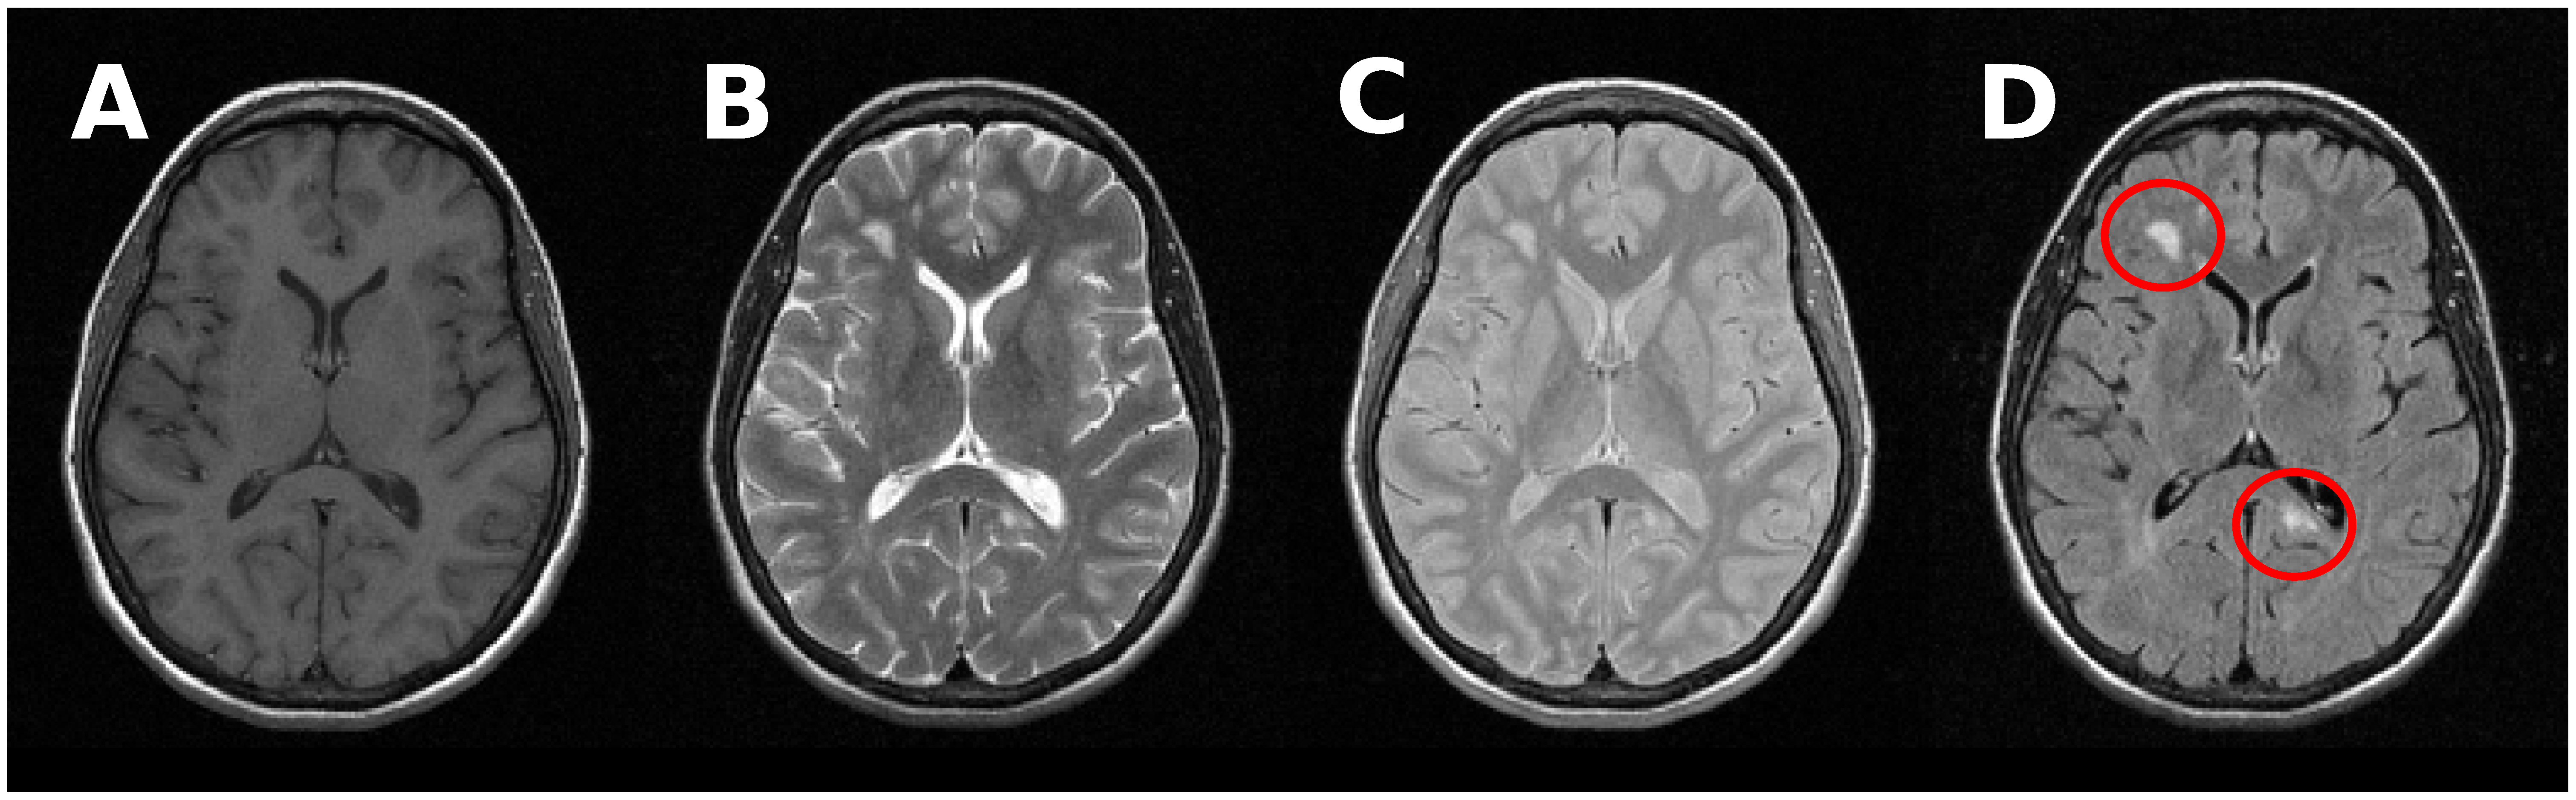
\includegraphics[width=1\textwidth]{figures/figure_1.eps}
  \end{center}
    \caption{MRI image modalities. A) T1-weighted (T1-w) image sequence. B) T2-weighted (T2-w) image sequence. C) Proton Density-weighted (PD-w) image sequence. D) Fluid Attenuated Inversion Recovery (FLAIR) sequence. MS plaques are shown inside red circles on the FLAIR modality. MS plaques are hypointense with respect to GM and WM in T2-w, PD-w and FLAIR sequences, while hypointense with respect to WM on the T1-w modality.}
    \label{mri_modalities}
\end{figure*}

In this aspect, new criteria for MS diagnosis and monitoring has been revised in the last years \cite{Polman2011}, due to the MRI sensitivity to reveal focal white matter (WM) lesions and disease activity in time and space \cite{Filippi2011}. Additionally, various studies have also analyzed the correlation between MRI brain tissue atrophy measures and MS disability status, showing that tissue loss is an important component of the disease progression \cite{Chard2002, Filippi2013, Fisher2008, Rudick2009}. Tissue loss seems to increase through the course of MS with a similar rate between 0.3\% and 0.5\% per year, and independently of the MS subtype \cite{DeStefano2010, Rudick2009}. In general, GM atrophy is more associated with disability changes than WM atrophy \cite{Fisniku2008}, and not only in the RRMS and SPMS MS subtypes \cite{Fisher2008, Rudick2009}, but also in Clinically Isolated Syndrome (CIS) patients where several studies have shown a significantly greater ventricular cavities and an associated GM loss on MRI scans of CIS patients that will develop MS compared to those who not \cite{Ceccarelli2010,Filippi2013}.

\subsection{Image analysis in MS}
\label{subsec:image_analysis}

Manual analysis of brain images is unfeasible in practice, given the large number of two-dimensional slices of each three-dimensional MRI patient image and the possible intra/inter observer variability between experts \cite{Cabezas2011}. This has led to the development since the early nineties of a wide number of lesion and tissue segmentation methods, with the aim to reduce the time of manual interaction and the inherent variability of manual annotations \cite{Cline1990, Gerig1992, Kapur1996}. 


\subsubsection{Pre-processing of MRI images}
Acquired brain MRI volumes incorporate non-brain tissue parts of the head such as eyes, fat, spinal cord or brain skull. Brain tissue extraction from non-brain tissue is commonly referred in the literature as skull-stripping (see Figure \ref{preprocessing_mri} B and C). Skull-stripping has a direct effect on the performance of automated methods, as differences in skull stripping would lead into unexpected results in the tissue classification if skull or eyes are included as brain tissue \cite{Acosta-Cabronero2008, Popescu2012}. Among the different proposed methods for skull-stripping \cite{Acosta-Cabronero2008, Lee2003, Roura2014}, the Brain Extraction Tool (BET) \cite{Smith2002} and the Brain Surface Extractor (BSE) \cite{Shattuck2001} are the most commonly used methods by the neuroimaging community.

Furthermore, inherent characteristics of the MRI acquisition process such as differences in the magnetic field, bandwidth filtering of the data or eddy currents driven by field gradients usually derive in image artifacts that may also have a negative impact on the performance of methods \cite{Simmons1994}. In these cases, intensity correction of MRI images is either performed before lesion/tissue segmentation, or as an integrated part of the tissue segmentation pipeline  (see Figure \ref{preprocessing_mri} D). Among the former available strategies proposed \cite{Arnold2001,Hou2006}, the N3 \cite{Sled1998} and N4 \cite{Tustison2010} methods are currently the most widely used tools used for intensity correction. 


\begin{figure*}[top]
  \begin{center}
    %\vspace{-3cm}
    \includegraphics[width=1.0\textwidth]{figures/figure_2.eps}
  \end{center}
    \caption{MRI pre-processing steps. A) T1-weighted (T1-w) image sequence. B) Computed brain mask using the BET approach \cite{Smith2002} and C) skull stripped T1-w sequence  . D) Estimated T1-w bias-field using the N3 method proposed by \cite{Sled1998}.}
    \label{preprocessing_mri}
\end{figure*}

\subsubsection{Automated lesion segmentation}

MRI based diagnostic criteria for MS has led to an increasing need to analyze quantitatively focal MS lesions in individual and temporal studies \cite{Cabezas2014, Polman2011}. Different sequences such as T2-w, PD-w and FLAIR are often used in lesion detection and segmentation, as MS lesions appear brighter than GM and WM on them. However, WM lesions often present a similar signal intensity profile to CSF on T2-w. In contrast, FLAIR sequences suppress fluids from the image, restraining the CSF tissue effects on the acquired image, although some severe T2-w hyperintense lesions appear similar to CSF in FLAIR \cite{Harmouche2015}. 

A wide number of automated lesion segmentation techniques have been proposed during the last years \cite{Garcia-Lorenzo2013, Llado2012}. In these methods, lesion segmentation is based either in supervised or unsupervised strategies. Supervised methods employ a training set of correctly-identified observations that are used as prior information to learn the lesion characteristics. Newer proposed strategies integrate spatial decision forest \cite{Geremia2011}, statistical methods \cite{Sweeney2013}, patch-based models \cite{Guizard2015} or adaptive dictionary learning strategies \cite{Deshpande2015}. In contrast, unsupervised learning methods do not use any prior information in the segmentation task, which involves grouping data into categories based on some measure of inherent similarity or distance characteristic of the input images. Among these, most recent methods include probabilistic models which separate WM lesions from normal-appearing tissue by considering lesions as an outlier class \cite{Harmouche2015,Jain2015,Tomas-Fernandez2015}, or techniques that make use of the signal intensity of lesions on FLAIR to apply several thresholding methods with post-processing steps to automatically segment lesions \cite{Roura2015, Schmidt2012}. 


\subsubsection{Automated brain tissue segmentation in MS}
\label{subsec:lesion_segmentation}
The existent correlation between brain tissue atrophy measures and MS disability status \cite{Filippi2013, Fisher2008}, has increased the necessity to develop robust automated brain tissue segmentation methods capable to perform accurate brain tissue volume measurements \cite{Giorgio2013}. However, automated segmentation of brain tissue is still a challenging problem due to the complexity of the images, existence of lesions, differences in tissue intensities, noise, intensity inhomogeneities and the absence of models of the anatomy that fully capture the possible deformations in each structure \cite{Cabezas2011, Kapur1996}. 

A wide number of brain tissue segmentation methods have been proposed so far. General purpose intensity based methods usually perform tissue segmentation on T1-w sequences, as this modality clearly separates gray matter from white matter. These include probabilistic strategies based on Bayesian inference \cite{Ashburner2005,Marroquin2002, Roy2012,Shattuck2001}, Markov Random Fields models \cite{Bricq2008, Tohka2010, Zhang2001}, or unsupervised clustering methods \cite{Caldairou2011, Pham2001}. In contrast, supervised learning approaches also combine T1-w sequences with other modalities such as T2-w and PD-w using \textit{K-Nearest-Neighbor} classifiers \cite{deBoer2009,Vrooman2013}, \textit{Support Vector Machines} \cite{Akselrod2006,Opbroek2013}, \textit{Random Forests} \cite{yi2009,Mahapatra2014}, or trained \textit{Gaussian mixture models} \cite{Rajchl2015}. 

However, different studies have shown that tissue abnormalities found in MS image patients such as WM lesions reduce the accuracy of tissue segmentation methods \cite{Battaglini2012, Chard2010}. Effectively, WM lesions on T1-w are hypointense with respect to normal-appearing WM, and  therefore, lesion voxels that are classified as GM are distorting the overall GM volume. However, lesion voxels may also have an effect in the observed differences in normal-appearing tissue. WM lesions which are actually classified as WM decrease the mean overall signal intensity of the WM, causing that GM voxels with signal intensities similar to WM lesions may be also miss-classified as WM.  In contrast, if WM lesions are classified as GM, normal-appearing WM voxels with signal intensities similar to lesions may be miss-classified as GM. 
 
\subsubsection{Lesion filling}
\label{subsec:lesion_filling}
In MS, hypointense WM lesions have to be pre-processed before tissue segmentation in order to reduce the effects of WM lesions on tissue segmentation. Historically, WM lesions have been masked-out of the T1-w before segmentation, and their volume have been added to WM afterwards \cite{Chard2002}. Although this method effectively reduces the error in tissue volume, it has been show in several studies that this approach is not optimal \cite{Battaglini2012, Chard2010}. 

In this aspect, several strategies have proposed to in-paint lesions on the T1-w with signal intensities of the normal-appearing WM before tissue segmentation \cite{Battaglini2012, Chard2010, Magon2014, Sdika2009}, a process which is usually known in the literature as lesion filling. However, most of the available lesion filling methods require manual delineations of lesions, which may be tedious, challenging and time-consuming task depending of the characteristics of the image \cite{Llado2012}. When available, lesion filling has demonstrated not only a significant reduction in the associated errors of WM lesions in tissue volume measurements \cite{Popescu2014}, but also in image registration \cite{Ceccarelli2012,  Diez2014, Sdika2009} and cortical thickness measurements \cite{Magon2014}. 

\section{Research background}
\label{sec:research_background}

This thesis is located within the framework of different research projects associated to the Computer Vision and Robotics Institute (VICOROB) of the University of Girona\footnote{http://vicorob.udg.edu}. VICOROB has been working on numerous medical image analysis projects since 1996, mainly in segmentation and registration of mammography images. Lately in 2009, the research group started a fruitful collaboration with several medical MS research teams with the aim to develop new automated techniques capable to segment MS lesions and to perform atrophy measurements that can be transferred to experts for clinical use. In particular, our research in the MS field has been carried out within the following research projects:

\begin{enumerate}

\item $[2009-2012]$ PI09/91918 ``SALEM: Segmentaci\'{o}n Autom\'{a}tica de Lesiones de Esclerosis M\'{u}ltiple en im\'{a}genes de resonancia magn\'{e}tica'' awarded by the Instituto Carlos III. 

\item $[2009-2012]$ VALTEC09-1-0025 ``SALEM: Eines per a la segmentaci\'{o} autom\`{a}tica de lesions d'Esclerosi M\'{u}ltiple en resson\`{a}ncia magn\`{e}tica'' awarded in 2009 by the Generalitat de Catalunya within the ``Projectes de valoritzaci\'{o} VALTEC''.

\item $[2015-2017]$ TIN2014-55710-R: NICOLE: ``Herramientas de neuroimagen para mejorar el diagnosis y el seguimiento cl\'{i}nico de los pacientes con Esclerosis M\'{u}ltiple" awarded in 2014 by the spanish call Retos de investigaci\'{o}n 2014.

\item $[2015-2019]$ BiomarkEM.cat: ``New technologies applied to clinical practice for obtaining biomarkers of  atrophy and lesions in magnetic resonance images of patients with multiple sclerosis''. Awarded in 2015 by the Fundaci\'{o} la Marat\'{o} de TV3.

\end{enumerate}

Since then, the research group has published original contributions in different fields such as image pre-processing \cite{Roura2014}, MS lesion segmentation \cite{Cabezas2014, Cabezas2014b, Llado2012, Roura2015}, temporal analysis \cite{Ganiler2014,Llado2012b}, image registration \cite{Diez2014, Roura2015b}, and tissue segmentation \cite{Cabezas2011}. All the works have been done in collaboration with different medical MS teams from:

\begin{itemize}

\item The Hospital Vall d'Hebron: Dr. Rovira, who is the director of the ``Unitat de Resson\`{a}ncia Magn\`{e}tica-Centre Vall d'Hebron" (URMVH) and has participated in numerous research projects funded by public and private institutions in the last few years, as well as Dr. Pareto and technicians Huerga and Corral. This group is part of the MAGNIMS network, a European network of centers that share an interest in the MS study through MRI.
 
	 \item The Cl\'{i}nica Girona / Hospital Santa Caterina: Dr. Vilanova and Dr. Barcel\'{o} are the codirectors of the ``Unitat de Resson\`{a}ncia Magn\`{e}tica" at the Cl\'{i}nica Girona and are members of several national and international radiology societies.
 
	\item The Hospital Josep Trueta: Dr. Rami\'{o}-Torrent\`{a}, who is the current coordinator of the "Unitat de Neuroimmunologia i Esclerosi M\'{u}ltiple", as well as Drs. Robles and Beltr\'{a}n, who work for the radiology unit.

\end{itemize}

\section{Objectives}
\label{sec:objectives}

As part of the SALEM, NICOLE and BiomarkEM.cat research project frameworks, the main goal of this thesis is: 

\begin{center}
	%\fbox{\parbox[c]{0.85\textwidth}{\textbf{the improvement of the current pipeline capable to detect and segment MS lesions in MRI and its integration in a standard platform.}}}
	\fbox{\parbox[c]{0.88\textwidth}{\textbf{to develop a novel fully automated brain tissue segmentation method capable of computing accurate tissue volume measurements on images of MS patients.}}}
\end{center}

Different stages have to be covered first in order to fulfill the main proposed goal. All them can be considered as sub-objectives that allow us to gain a better knowledge of the different parts that compose a fully automated tissue segmentation method for MS images containing lesions. In what follows, we detail these proposed sub-goals: 

\begin{itemize}

\item \textbf{to analyze the state-of-the-art of tissue segmentation methods}. This stage aims to review the different proposed tissue segmentation techniques in order to understand their advantages and drawbacks. Methods are evaluated on public databases that incorporate manual tissue annotations, which allows to perform a quantitative analysis of the accuracy of the methods.
  
\item \textbf{to study the effect of WM lesions on tissue segmentation of MS patient images}. Although it is know that the inclusion of WM lesions on tissue segmentation distort the brain volume measurements, this effect has not been studied and compared across different tissue segmentation methods. In this aspect, the second stage is focused on the analysis of the effects of WM lesions on the tissue distributions of a set of tissue segmentation approaches using multi-center 1.5T MS data from different scanners. Our hypothesis here is that a better knowledge of the correlation between lesion attributes, such as signal intensity and lesion size, and the observed differences in tissue volume of the analyzed algorithms may be beneficial to design a tissue segmentation method for MS. 

\item \textbf{to reduce the effect of WM lesions on tissue segmentation of MS patient images designing and implementing a new lesion filling algorithm}. As said in section \ref{subsec:lesion_filling}, WM lesions have to be pre-processed before tissue segmentation in order to reduce the effects of those lesions on tissue segmentation. In this regard, the third sub-goal is two-fold: firstly, to compare the accuracy of different lesion filling techniques proposed in the literature, analyzing their accuracy on both 1.5T and 3T databases. 

Secondly, after analyzing the benefits and drawbacks of each proposed method, we aim to propose a new lesion filling algorithm in order to overcome the possible limitations of existent methods.

\item \textbf{to analyze the effect of automated algorithms that perform WM lesion segmentation and filling on the tissue segmentation}. Although lesion filling techniques have already been successfully applied to reduce the effect of WM lesions on tissue segmentation, usually WM lesions are annotated manually before tissue segmentation. In contrast, the effect of both automated lesion segmentation and filling on tissue segmentation is still unclear. The fourth stage of the thesis aims to understand the effects of the inherent errors in automated lesion segmentation on the posterior lesion filling and tissue segmentation. Thus, we aim to compare the accuracy of different state-of-the-art  pipelines that incorporate automated lesion segmentation, lesion filling and tissue segmentation on MS data. Furthermore, we analyze the extend of the effect of remaining WM lesions on the differences in tissue segmentation, which may be beneficial to update the knowledge gained in previous stages. 

\item \textbf{to propose a new fully automated tissue segmentation method for MS patient images}. Finally, we aim to benefit from the stages to propose a novel \textbf{fully automated tissue segmentation method} able to deal with images of MS patients with different level of brain atrophy and lesion load. In this last stage, we aim to validate the accuracy of the proposed method by comparing it with the state-of-the-art in tissue segmentation in MS. 

\end{itemize}

\noindent This objective refers to the brain tissue segmentation of MS patient images into GM, WM CSF in transversal studies. We do not concentrate in differences in tissue volume at different stages, but in the effect of WM lesions in the final tissue segmentation. All these stages will be carried out using not only public databases but also different 1.5T and 3T databases of MS patients from the collaborating hospital centers. \textbf{Furthermore, as part of the goals of the research frameworks from which this thesis is located, implementations of all the proposed methods will be publicly available for the research community}.

\subsection{Document structure}
\label{sec:label}

A graphical description of the structure of the thesis linking all the chapters presented is shown in Figure \ref{document_structure}. Connections between the chapters depict the conceptual link between them. The rest of the document is organized as follows:

\begin{figure*}[top]
  \begin{center}
%    \vspace{-3cm}
    \includegraphics[width=1\textwidth]{figures/document_schema.eps}
  \end{center}
    \caption{Organization of the document. Preliminary chapter 1 describes the research context and the main objectives of this thesis. Chapters 2 to 6 introduce the main contributions of this work based on the different works submitted or published in research journals. Chapter 7 presents a general discussion of the results obtained from Chapters 2 to 6. Finally, the main conclusions and the proposed future work are presented in Chapter 8. Connections between chapters depict a conceptual link between them.}
    \label{document_structure}
\end{figure*}


\begin{itemize}
%\item \textbf{Chapter 1. Introduction.} This chapter has described the research context and the main objectives of this thesis.
\item \textbf{Chapter 2. Comparison of 10 brain tissue segmentation methods using revisited IBSR annotations.}  We present here comprehensive comparison of the accuracy of 10 brain tissue segmentation methods on two public MRI databases. This chapter is based on the paper published in  the\textit{ Journal of Magnetic Resonance Imaging} in 2015. 

\item \textbf{Chapter 3. Evaluating the effects of white matter multiple sclerosis lesions on the volume estimation of 6 brain tissue segmentation methods.} After reviewing different tissue segmentation techniques using public data, we perform a detailed analysis of the effects of WM lesions on the brain tissue volume measurements of six of these tissue segmentation methods using MS data from different hospital centers collaborating in the research projects. This chapter is based on the paper published in  the \textit{American Journal of Neuroradiology} in 2015. 

\item \textbf{Chapter 4. A white matter lesion-filling approach to improve brain tissue volume measurements.} In this chapter, we propose a new technique to fill WM lesions on 1.5T and 3T data, validating its accuracy with respect to other methods in the literature. This chapter is based on the paper published in the \textit{NeuroImage: Clinical} journal in 2014. 

\item \textbf{Chapter 5. Quantifying brain tissue volume in multiple sclerosis with automated lesion segmentation and filling.} In this chapter we present a detailed  evaluation of the performance of different automated pipelines that incorporate lesion segmentation, lesion filling and tissue segmentation on MS data. This analysis is novel in the sense that this is the first work that evaluates two automated pipelines on MS data. This chapter is based on the paper published in the \textit{NeuroImage: Clinical} journal in 2016.

\item \textbf{Chapter 6. Automated brain tissue segmentation of MR images in the presence of white matter lesions.} We propose here a novel fully automated tissue segmentation pipeline designed to deal with MS patient images containing lesions. We validate the accuracy of the proposed method comparing the performance with other state-of-the-art techniques. Data from the MRBrainS13 challenge as well as data from our hospital collaborators is used to perform the evaluation. This chapter is based on the paper submitted to the \textit{Medical Image Analysis} journal in 2016.  

\item \textbf{Chapter 7. Results and discussion.} This chapter provides a comprehensive discussion of the results obtained in this thesis.
\item \textbf{Chapter 8. Conclusions and future work.} Finally, the main conclusions based on the contributions of this thesis are defined. Based on these conclusions, we  also point out different future works to improve and extend the work carried out in this thesis.   
\end{itemize}

%%% Local Variables:
%%% mode: latex
%%% TeX-master: "../main"
%%% End:


\chapter{Comparison of 10 brain tissue segmentation methods using revisited IBSR annotations.}  
\label{chapter:chapter_2}

In this chapter, we perform a quantitative evaluation of the accuracy of 10 automated brain tissue segmentation methods. The methods are compared using the Internet Brain Segmentation Repository (IBSR) databases IBSR20 and IBSR18 \footnote{https://www.nitrc.org/projects/ibsr/}. The performance of these methods is then evaluated by ranking their accuracy based on their significant differences with respect to the other methods. This proposed evaluation has been published in the following paper:

\vspace{2cm}

\noindent\fbox{\parbox[b]{\linewidth}{Paper published in the \textbf{Journal of Magnetic Resonance in Medicine} (JMRI)

Volume: 41, Issue: 1, Pages: 93-101, Published: January 2015

DOI: 10.1002/jmri.24517

Quality Index: 3.21 (Quartile 1)}}
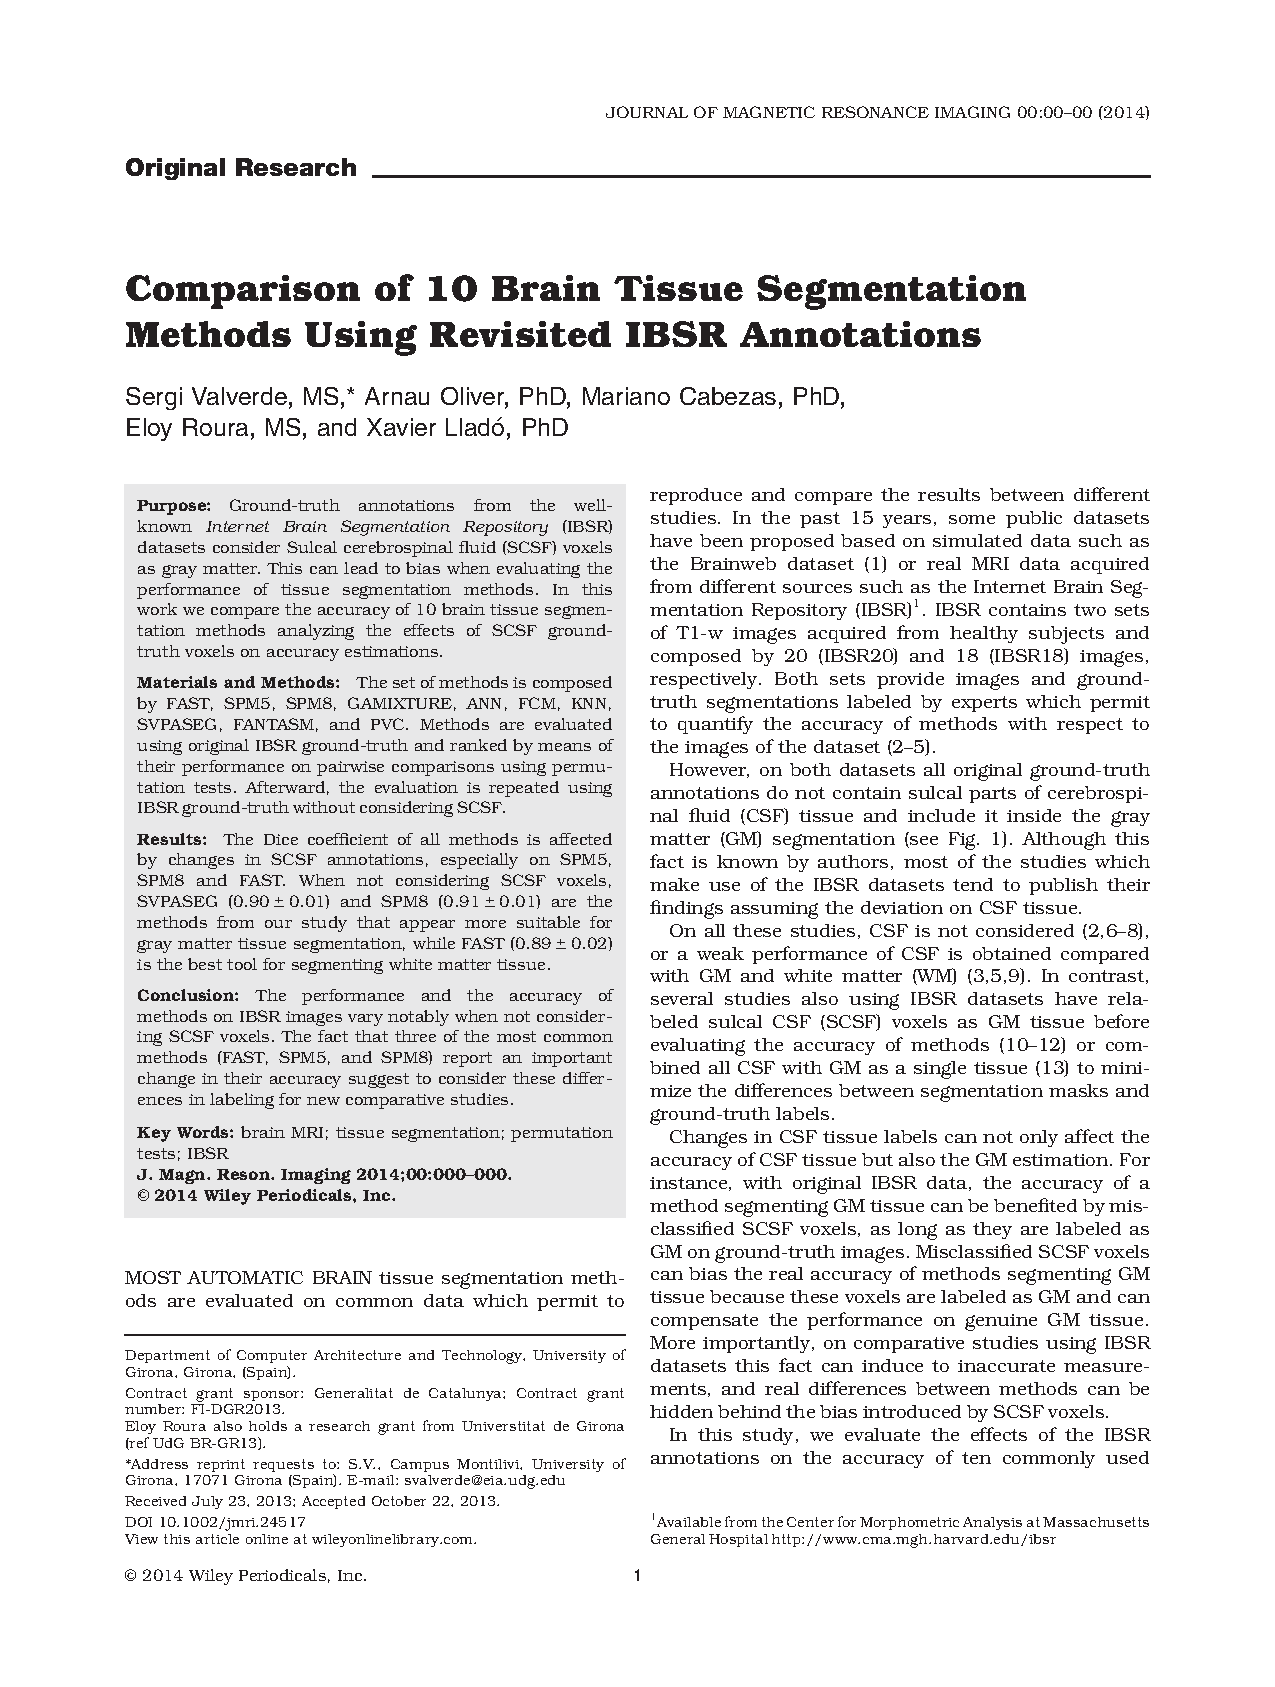
\includepdf[pages={-}]{./papers/jmri2014.pdf}


%%% Local Variables:
%%% mode: latex
%%% TeX-master: "../main"
%%% End:




\chapter{Evaluating the effects of white matter multiple sclerosis lesions on the volume estimation of 6 brain tissue segmentation
methods}  
\label{chapter:chapter_3}
In this chapter, we present a study of the impact of MS white matter lesions on the brain tissue measurements of six well-known segmentation techniques. These include straightforward techniques such as Artificial Neural Network (ANN) and fuzzy C-means (FCM) as well as more advanced techniques like the Fuzzy And Noise Tolerant Adaptive Segmentation Method (FANTASM), FMRIB's Automated Segmentation Tool (FAST), and Statistical Parametric Mapping (SPM) with versions SPM5 and SPM8. This proposed evaluation has been published in the following paper:

\vspace{2cm}

\noindent\fbox{\parbox[b]{\linewidth}{Paper published in the \textbf{American Journal of Neuroradiology} (AJNR) 

Volume: 36, Pages: 1109-1115, Published: February 2015

DOI: 10.3174/ajnr.A4262

JCR RNMMI IF 3.589, Q1(19/125)
}}
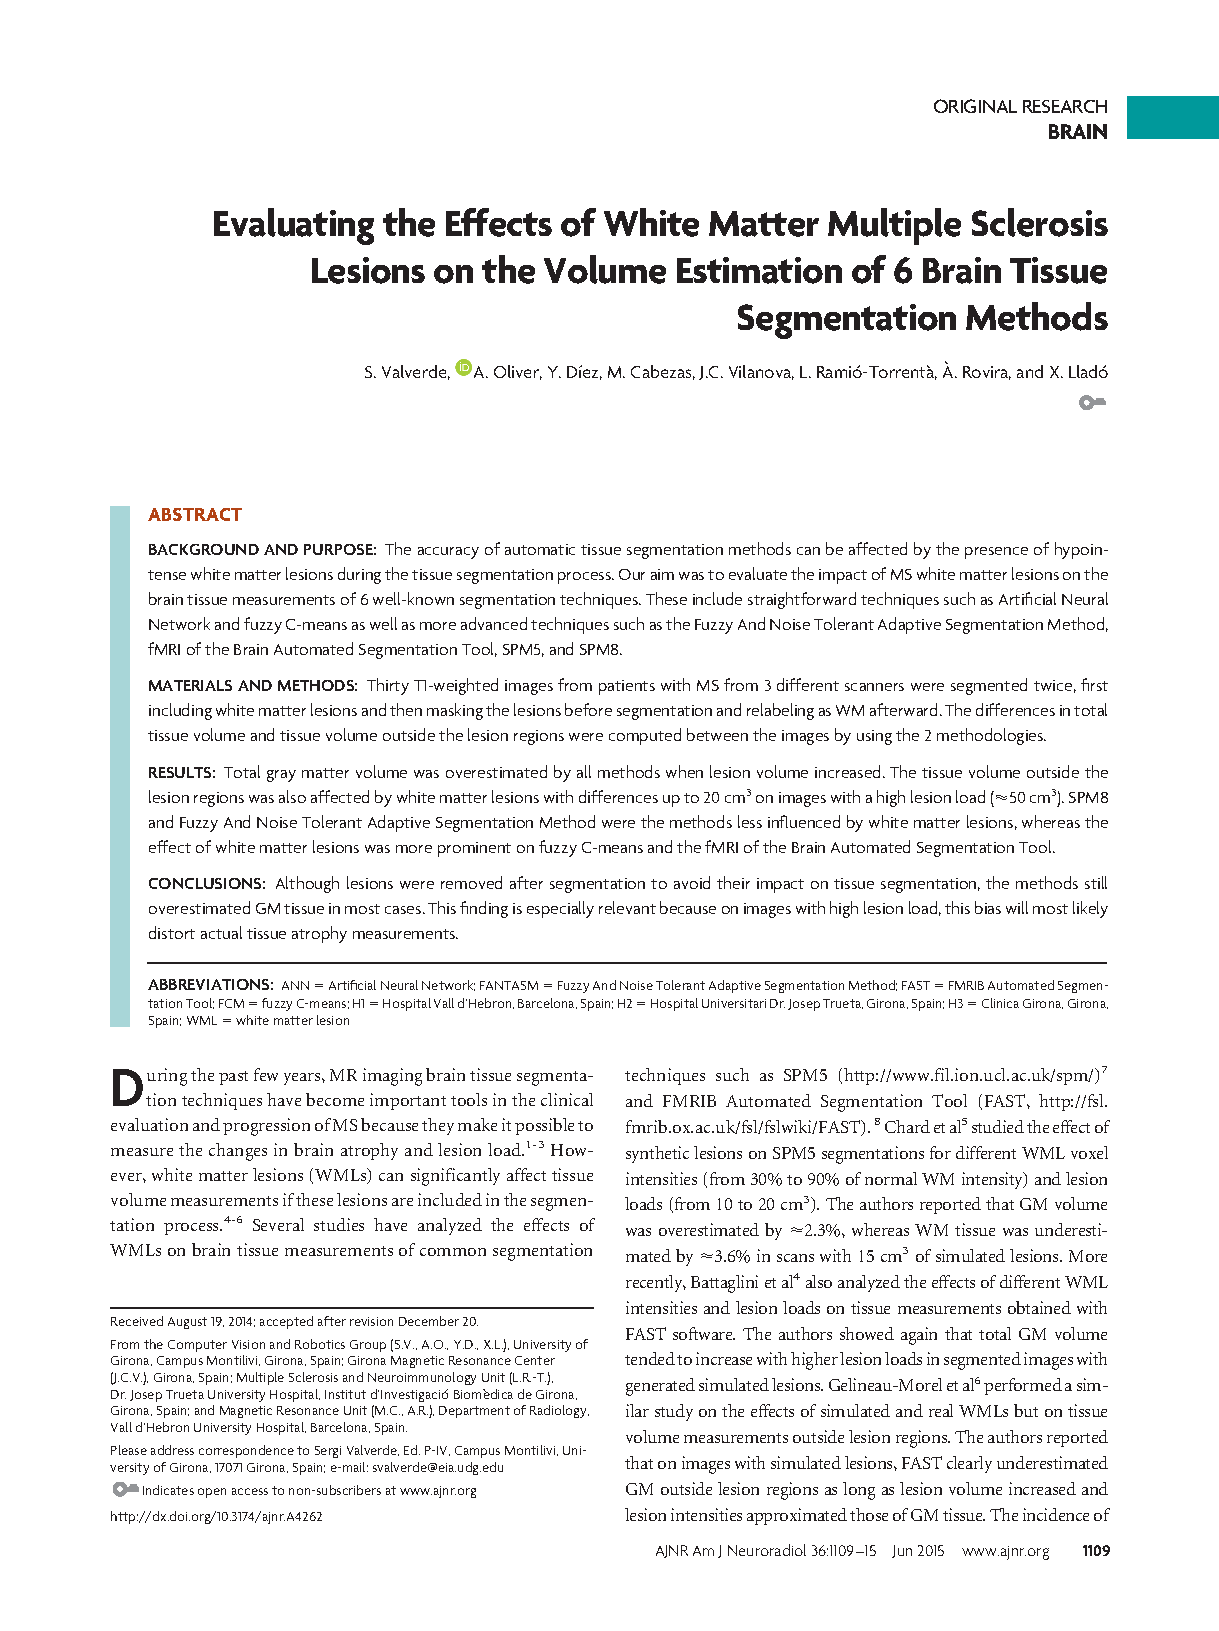
\includepdf[pages={-}]{./papers/ajnr2015.pdf}


%%% Local Variables:
%%% mode: latex
%%% TeX-master: "../main"
%%% End:




\chapter{A white matter lesion-filling approach to improve brain tissue volume measurements.}

\label{chapter:chapter_4}

In this chapter, we propose a new technique to fill WM lesions before tissue segmentation. The proposed approach is evaluated in both 1.5T and 3T data. We validate our method comparing its accuracy with other proposed automated lesion filling methods on the same data. Furthermore, the proposed technique has been released for public use both as a standalone program or as SPM8/SPM12 library.  
This work has been published in the following paper:

\vspace{2cm}

\noindent\fbox{\parbox[b]{\linewidth}{NeuroImage: Clinical

Volume: 6,  Pages: 86-92, Published: August 2014

DOI: 10.1016/j.nicl.2014.08.016

Quality Index: 2.53 (Quartile 2)}}
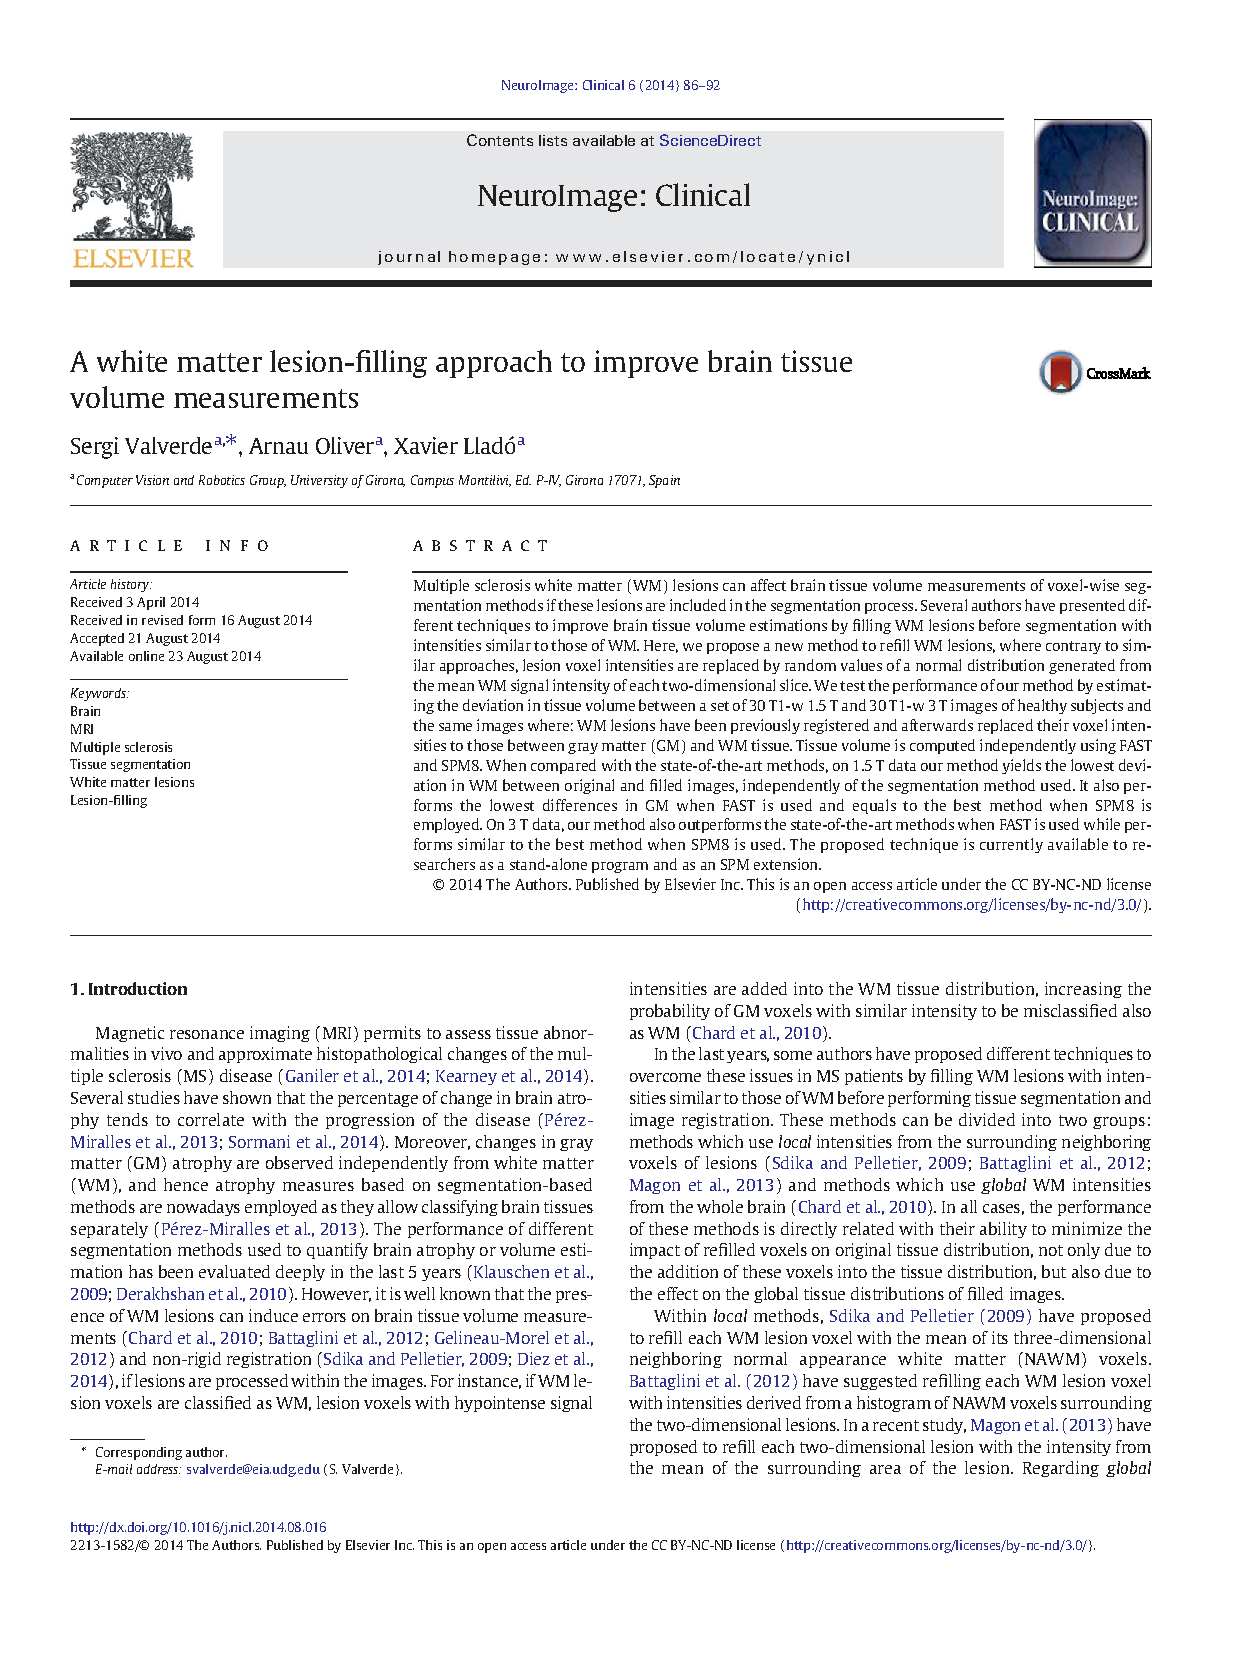
\includepdf[pages={-}]{./papers/nicl2014.pdf}

%%% Local Variables:
%%% mode: latex
%%% TeX-master: "../main"
%%% End:




\chapter{Quantifying brain tissue volume in multiple sclerosis with automated lesion segmentation and filling}  

\label{chapter:chapter_5}

In this chapter, we present a detailed evaluation of the performance of different pipelines that incorporate fully automated processes such as lesion segmentation, lesion filling and tissue segmentation on MS data. For each automated pipeline, we analyze the percentage of error in tissue segmentation between a set of 70 MS images, where WM lesions have been refilled before segmentation and the same images processed at different levels of automation from manually masking lesions to fully automated lesion segmentation and filling. This analysis has been published in the following paper:

\vspace{2cm}

\noindent\fbox{\parbox[b]{\linewidth}{Paper published in the \textbf{NeuroImage: Clinical} journal (NICL)

Volume: 9,  Pages: 640-647, Published: October 2015

DOI: doi:10.1016/j.nicl.2015.10.012

JCR N IF 2.526, Q2(6/14)}}
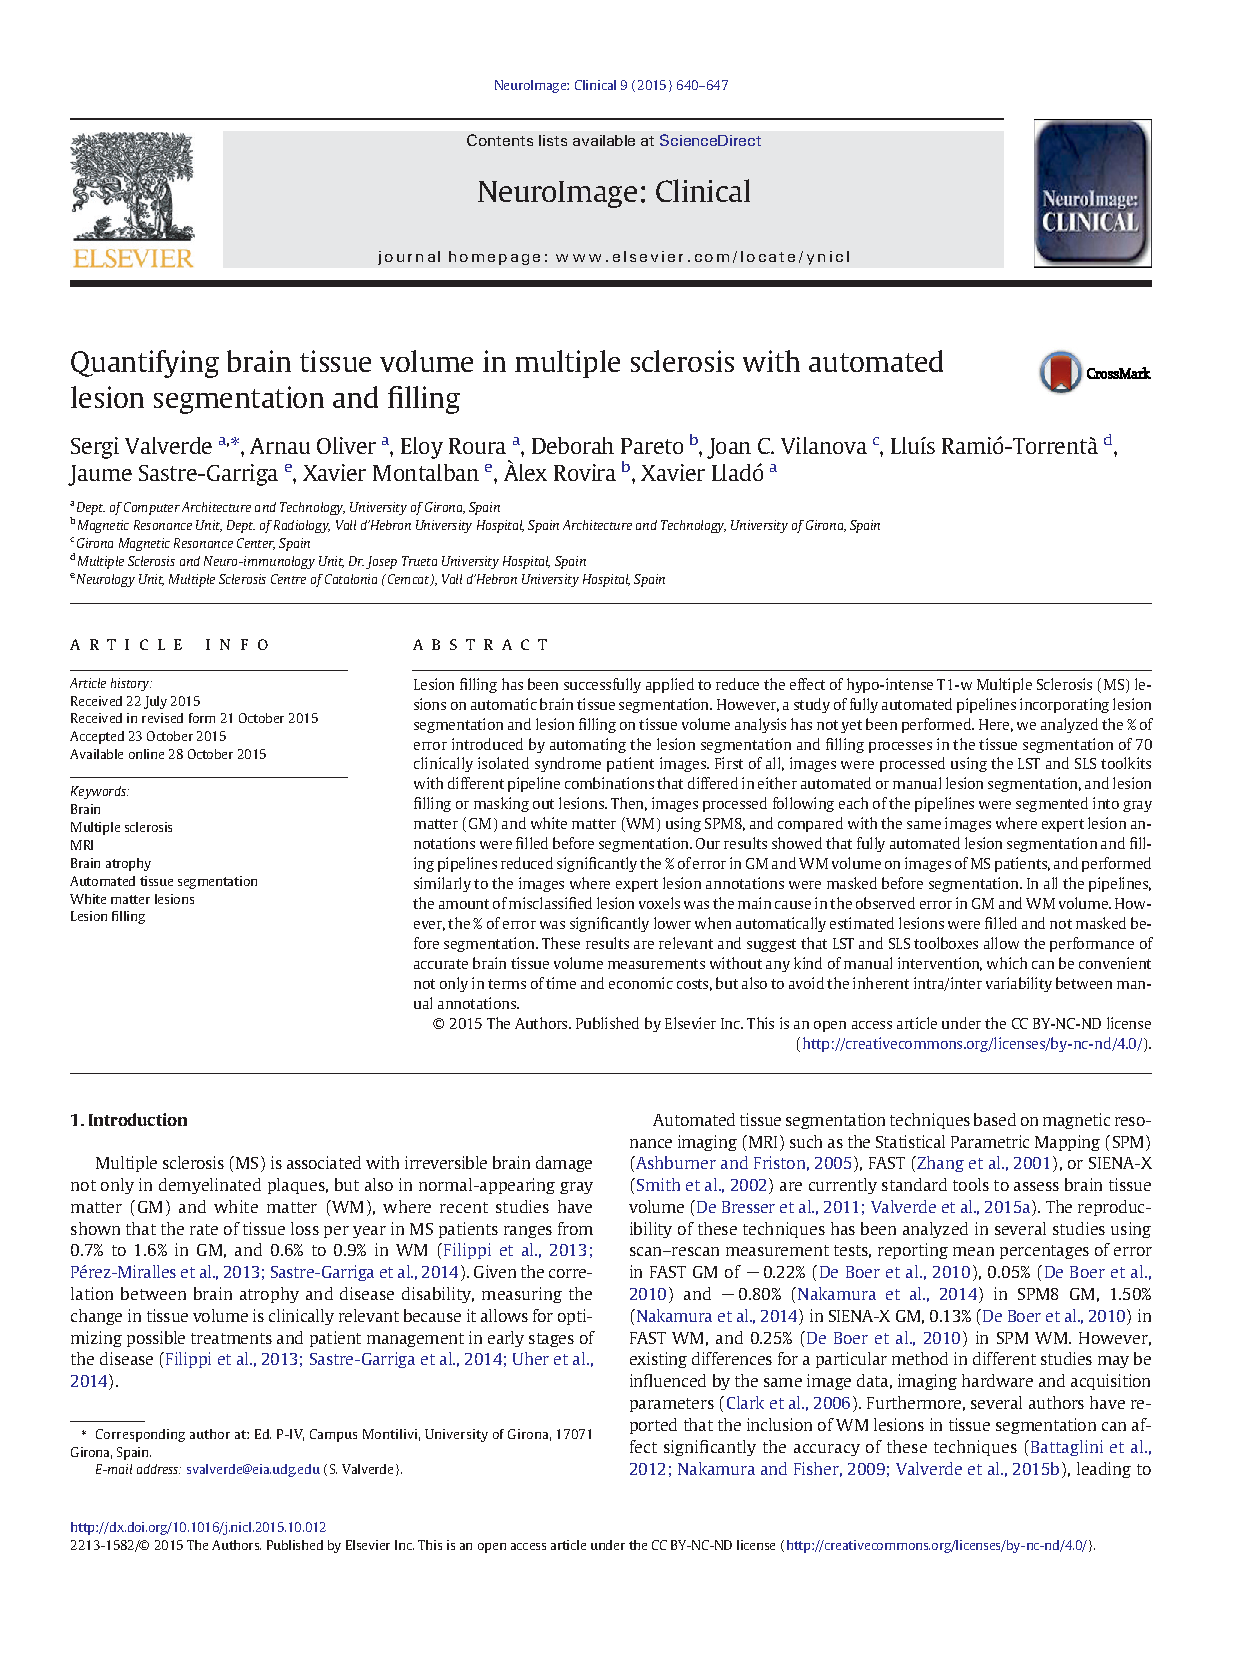
\includepdf[pages={-}]{./papers/nicl2015.pdf}


%%% Local Variables:
%%% mode: latex
%%% TeX-master: "../main"
%%% End:




\chapter{Automated tissue segmentation of MR brain images in the presence of white
matter lesions.}  

\label{chapter:chapter_6}

In this chapter, we propose a novel automated pipeline for tissue segmentation of 
MS patient images containing lesions. The accuracy of the method is evaluated using both the challenge MRBrainS13 database\footnote{http://mrbrains13.isi.uu.nl/} and a 3T MS database of MS patient images. We validate the accuracy of the proposed method with other state-of-the-art techniques. A public version of the method has been released for public use.  The proposed pipeline has been described in detail in the next paper and submitted to the Medical Imaging Journal:

\vspace{2cm}

\noindent\fbox{\parbox[b]{\linewidth}{Paper submitted to the\textbf{ Medical Image Analysis }(MIA) journal

Currenly in revision.

Quality Index: 3.68 (Quartile 1)}}
\includepdf[pages={-}]{./papers/mia2016.pdf}
%\includepdf[pages={-}]{./papers/msseg_review.pdf}


%%% Local Variables:
%%% mode: latex
%%% TeX-master: "../main"
%%% End:





\chapter{Main results and discussion}
%\addcontentsline{toc}{chapter}{Main results and discussion} 

MRI tissue segmentation techniques are being used increasingly as standard tools to assess brain tissue volume. However, automated tissue segmentation is still a challenging task in MS, due to the tissue abnormalities found in MS patient images such as WM lesions that are known to reduce the accuracy of tissue segmentation methods. When expert manual annotations of WM lesions are available, lesion filling has shown to be an effective method to reduce the effects of those lesions on tissue segmentation. However, manual annotations are time-consuming and prone to variability among experts, which in combination with the need to analyze focal MS lesions quantitatively in individual and temporal studies, has led to the development of a wide number of automated lesion segmentation of MS lesions. Therefore, a solid understanding of the effects of MS lesions on automated pipelines that concatenate processes such as lesion segmentation, lesion filling and tissue segmentation is important. 

As stated in section \ref{sec:objectives}, each of these processes covers a part of the necessary knowledge needed to accomplish the goal of this thesis. This chapter provides a comprehensive discussion of the main results shown in previous chapters, analyzing each of these necessary processes for the development of a fully automated tissue segmentation method for MS images.

\section{Effect of WM lesions on tissue segmentation}

A wide number of automated tissue segmentation methods have been proposed in the literature so far. In Chapter \ref{chapter:chapter_2}, we evaluated the accuracy of ten approaches using the two available public databases of healthy subjects, IBSR18 and IBSR20. With the aim of including a wide set of different segmentation approaches and available tools, the analysis included well-known implementations of image segmentation algorithms such as ANN, FCM, and KNN, as well as available public toolboxes such as FAST, SPM5, SPM8, PVC, GAMIXTURE, SVPASEG, and FANTASM. Results were presented before and after correcting the CSF masks, as we saw that available annotations ignored sulcal CSF tissue in the original masks. When sulcal CSF was corrected, the SVPASEG, SPM8 and FAST yielded the highest accuracy with both databases.  However, most of the methods were not robust against changes in acquisition sequences, intensity inhomogeneities and special attributes of the two databases,  which highlighted the fact that the brain tissue segmentation problem was still open, because there was not a single method that achieved a significantly higher accuracy with all tissues. 

Afterwards, six of these methods (ANN, FCM, FANTASM, FAST, SPM5 and SPM8) were evaluated on MS data from different hospital centers and scanners in order to analyze the extent to which tissue volume estimations were affected by changes in the WM lesion volume and intensity. Our results showed that the SPM8 had the lowest differences in total volume, while the FANTASM and again, the SPM8 were the methods where the incidence of WM lesions was the lowest on normal-appearing tissue. In general, the differences in tissue volume were lower for methods combining morphological prior information, namely the SPM5 and SPM8, or spatial constraints, like the FANTASM and FAST. In contrast, these differences were higher on simpler intensity based algorithms such as FCM and ANN, that lacked spatial correction. This fact and the higher performance on healthy data of former methods, stressed the necessity of adding morphological prior information and/or spatial constraints to the automated brain tissue segmentation, not only to overcome inherent MRI bias field artifacts but also as an important component to deal with WM lesions.

The main factor in the differences in tissue volume across the methods was caused by lesion volume. Furthermore, WM lesion voxels tended to be classified as GM in images where the variation between the lesion signal intensity and the mean signal intensity of normal-appearing WM was higher, which indicated a direct relationship between the differences in the brain tissue volume and the changes in the lesion load and WM lesion intensity. However, the lesion voxels also had a direct effect on the differences in GM and WM outside the lesion regions. As already mentioned in Chapter \ref{chapter:chapter_3}, these differences are especially important because they highlight the bias introduced by WM lesions on the estimation of tissue volume that is not pathologically affected. Our analysis showed that if lesion voxels were not considered in the computation of the brain volume, methods would still tend to overestimate GM, especially in images with a higher lesion load. 
The observed differences in normal-appearing tissue volume were important. Although lesion voxels could be reassigned to WM after segmentation, part of the bias was still present if these lesions were present in image segmentation.

Furthermore, differences in the total tissue volume may be canceled between the errors produced in the same lesion regions as well as the effect of these voxels on normal-appearing tissue. This fact clearly shows the necessity of either processing WM lesions before segmentation or modeling them as part of the tissue segmentation formulation. 


\section{Effect of lesion filling in tissue segmentation}

Over the last few years, different techniques have been proposed to reduce the bias introduced by WM lesions on the brain tissue volume measurements in MS images, mostly by in-painting WM lesions on T1-w with signal intensities similar to normal-appearing WM.  After reviewing the  available related literature in Chapter \ref{chapter:chapter_4}, we classified the existing methods into groups, those that filled WM lesions using the \textit{local} intensities from the surrounding neighboring lesion voxels, and those that used \textit{global} WM intensities from the whole brain to fill WM lesions. Although all these methods had already been validated separately, we performed a general comparison of all the available techniques in order to analyze their accuracy with the same 1.5T and 3T data and also to investigate their performance with different tissue segmentation techniques such as the FAST and SPM8.

This analysis served as a basis for a new technique to refill WM lesions that was a compromise between \textit{global} and \textit{local} methods. Our proposed method filled lesion voxel intensities with random values of a normal distribution generated from the mean WM signal intensity of each two-dimensional slice. Contrary to \textit{local} methods, where lesions were refilled with signal intensities coming from surrounding WM voxels, our approach was capable to reproduce better the original WM tissue distribution on images with high lesion load, because lesion voxels were refilled using random signal intensities from all the WM voxels of the slice. Although on our approach the probability of each tissue was first estimated using a clustering three-dimensional segmentation, we found that filling lesions with signal intensities from the same slice was more appropriate, as this approach reproduced better the intensity distribution of WM tissue at each slice than using the global three-dimensional intensity profile.

Our results showed that when compared to other methods, our approach yielded the lowest deviation in GM and WM volumes with 1.5T and 3T data when the FAST tissue segmentation was used. When the SPM8 tissue segmentation method was used, the performance of our lesion filling method was also very competitive, yielding the lowest differences or similar to those of the best method in GM and WM. In contrast to the rest of the pipelines, differences in tissue volume between the same images filled with our method and afterwards segmented with either the FAST or SPM8 were very low ($<0.1\%$), which indicates that the proposed strategy was equally efficient independently of the tissue segmentation chosen.

The proposed algorithm performed significantly better than \textit{local} methods on images with higher lesion loads. In contrast to \textit{global} methods, \textit{local} methods may be limited by the range of similar intensities coming from neighboring voxels, which on images with large lesions may introduce a bias on GM and WM tissue distributions by the addition of a considerable number of voxels with similar intensities. Furthermore, the performance of our approach was also better on images with high lesion loads when compared with \textit{local} methods, specially on images with lower resolution such as 1.5T data, most probably because our method estimated the mean global normal-appearing WM intensity for each slice independently, being sensitive enough to reproduce possible changes in the intensities between slices.


\section{Effect of automating lesion segmentation and filling on  tissue segmentation}
\label{sec:label}

As already mentioned earlier, lesion filling has proven to be an effective method to reduce the effects of these lesions on tissue segmentation. However, in all the lesion-filling approaches, including ours, MS lesions have to be known a priori, which requires delineating lesions manually. This is a clear limitation in terms of fully automatizing brain tissue in the presence of MS lesions, which motivated the evaluation of the effect of automated lesion segmentation on tissue segmentation. Although different automated tissue segmentation methods have been proposed, most are based on supervised learning, which requires explicit training, usually with a large amount of labeled data. Labeled data may be not available, which increased the interest of the community in unsupervised methods that can operate without prior data. As shown in Chapter \ref{chapter:chapter_5}, we compared two pipelines that combined automated lesion segmentation and filling as a first step to understand the effect of fully processed images on tissue segmentation. 
 
Given the performance shown in our previous studies and its wide use in clinical studies, the SPM8 was used as a reference tissue segmentation method to measure tissue volume on a set of 70 3T images from CIS patients. On these images, available manual expert annotations were employed to refill WM lesions before segmentation using the pipeline's filling method, and were considered as the ground-truth. Afterwards, we evaluated the differences in the GM and WM volumes between the set of filled images using manual annotations and the same images processed using different variations of the SLS and LST toolkits that differed in the level of manual intervention. Evaluating different pipelines with distinct levels of automation  permitted us to analyze the effect of each of the automated processes involved in the differences in the total and normal-appearing tissue volumes.  

As already stated in Chapter \ref{chapter:chapter_3}, this new analysis showed that the effect of lesions on the total tissue volume was limited due to a canceling effect between the errors produced in the same lesion regions, and the effect of these voxels on normal-appearing tissue. In all the pipelines that incorporated automated lesion segmentation, most of the differences observed in normal-appearing tissue were produced by the effect of false positive lesion voxels that were already segmented and had not been refilled. In contrast, there was no relevant correlation between the number of false positive lesion voxels and the differences observed in normal-appearing GM and WM, which suggested that most of these misclassified voxels were actually WM before refilling. The relationship between errors in automated lesion and tissue segmentation also suggest the importance of not only continuously reducing the number of missed lesions, but also stressing the necessity of contextual spatial information of lesion regions in order to confine them in the WM and, hence, reduce the effect of miss-classified voxels on the tissue segmentation.

As shown in the results presented in Chapter \ref{chapter:chapter_4}, masking-out lesion voxels before tissue segmentation might not be optimal, as leaving lesion voxels out of the tissue distributions appears to increase the differences in tissue volume with respect to lesion filled images, even if these voxels are re-assigned to WM afterwards. However, although not optimal, masking lesions before segmentation has proven to be a valid alternative to reduce the effects of WM lesions on research and clinical settings, and as a result in recent years, lesion filling techniques have already been applied on research and clinical studies. Regarding this, our results show that at least with the evaluated data, the differences in tissue volume between images where expert lesion masks have been masked-out and the same images where lesions have been automatically segmented and filled, are similar to images with a low lesion load $(<10ml)$. In contrast, from our experiments we observed that differences in tissue volumes tend to increase with the lesion load on masked-out images, while the increase of the error is more moderate in  fully-automated images. However, given the data available and the maximum lesion load considered in our analysis ($<20ml$), these findings should be considered with care. 

In any case, our analysis points out the fact that automated lesion segmentation and filling methods significantly reduced the impact of WM lesions on tissue segmentation, and had a similar performance to the pipelines that required manual expert intervention. These results are relevant and validate that each of these automated processes can be useful not only in terms of time and economic costs, but also as active processes in fully automated tissue segmentation in the presence of WM lesions.

\section{Fully automated tissue segmentation of images containing WM lesions}
\label{sec:label}

Previous sections of this thesis have stressed the advantages of dealing with MS lesions before the tissue segmentation, showing several general insights that can be useful for automated tissue segmentation of images containing lesions. The results obtained for the different methods evaluated in Chapters \ref{chapter:chapter_2} and \ref{chapter:chapter_3} have pointed out the superiority of methods that benefited from morphological prior information or spatial constraints in automated brain tissue segmentation. More importantly, the results obtained in Chapter \ref{chapter:chapter_3} have evidenced the effect of WM lesion on tissue segmentation and the necessity of dealing with MS lesions in order to reduce not only the bias produced by the same lesions but also the effect of these lesion voxels on normal-appearing tissue. In this scenario, we have proposed a new lesion filling technique that is very competitive with different databases and tissue segmentation methods, as shown in Chapter \ref{chapter:chapter_4}. Finally, we have shown in Chapter \ref{chapter:chapter_5} that the addition of unsupervised lesion segmentation and filling to already existing tissue segmentation pipelines significantly reduced the error in tissue volume when compared with other pipelines where lesions were segmented as normal tissue. 

Following these insights, we have developed a new, multi-channel method designed to segment brain tissues in MRI images of MS patients. As explained in Chapter \ref{chapter:chapter_6}, this approach makes use of a combination of intensity, anatomical and morphological prior maps to guide the tissue segmentation. Tissue segmentation has been tackled based on a robust partial volume segmentation where WM outliers have been estimated and refilled before segmentation using a multi-channel post-processing algorithm integrating  partial volume segmentation, spatial context, and prior anatomical and morphological atlases. Furthermore, the proposed method takes advantage of new affordable processors, such as GPUs, that reduce up to four times the execution time to register and segment tissue when compared to general purpose CPUs. This property makes this method useful for studies containing a large number of subjects to analyze.   

The proposed method has been quantitatively and qualitatively evaluated using different databases of images containing WM lesions. In order to analyze the extent to which the T1-w and FLAIR modalities intervened in the accuracy obtained, the proposed method was run in all the experiments using only the T1-w or using both the T1-w and FLAIR image sequences. As shown by the results, the proposed technique yielded competitive and consistent results in both general and MS specific databases without parameter tweaking. In the MRBrainS tissue segmentation challenge\footnote{http://mrbrains13.isi.uu.nl/}, our method, combining both T1-w and FLAIR, was the best non-supervised technique in the challenge, being ranked in 7th position out of 31 participant methods. When only the T1-w modality was used, the accuracy of the proposed method was still clearly superior to  methods such as FAST (ranked 21th) and SPM12 (best ranked 17th), even when they used both image modalities. With MS data, the performance of our method, combining the T1-w and FLAIR sequences, was similar to or better than the best evaluated pipeline incorporating lesion segmentation and filling. Differences in tissue volume between images processed with the proposed algorithm and the same images where lesions were filled using expert lesion annotations were lower than $0.15\%$ on all tissues, validating the overall capability of the proposed method reducing the effects of WM lesions on tissue segmentation. 

In general, our results showed that the percentages of error in tissue volume of our approach were low or similar with both databases. The percentages of error were lowest when the FLAIR modality was used, which evidences that this image sequence has a direct effect on the efficiency of the algorithm, and, consequently, it should be used when available. However, the accuracy of the method using only the T1-w modality was also superior to other strategies not designed to deal with MS lesions, which also evidences that the improvement in tissue segmentation was not only generated by the addition of the FLAIR modality, but also by the combination of intensity, anatomical and morphological priors, and the use of a specific outlier algorithm with integrated lesion filling.


%%% Local Variables:
%%% mode: latex
%%% TeX-master: "../main"
%%% End:

%Conclusions

\chapter{Conclusions}
% also add contributions

This thesis synthesizes our work done during the last three years. Following the same objectives defined in the Introduction chapter, we summarize in what follows the main conclusions and contributions of this thesis: 

\begin{itemize}

\item We analyzed and evaluated the state-of-the-art of brain tissue segmentation methods. This first stage aimed to quantitative review and evaluate different proposed tissue segmentation techniques in order to understand their advantages and drawbacks. As part of the resulting analysis published in the\textit{ Journal of Magnetic Resonance Imaging} in January of 2015,  
\textbf{our results showed a higher accuracy on several methods that incorporated morphological prior information and/or spatial constraints such as FAST, SPVASEG and SPM8. These methods were also less prone to changes in acquisition sequences and intensity inhomogeneities}.

\item We studied the effect of WM lesions on tissue segmentation of MS patient images. The second stage to cover was focused on the analysis of the effects of WM lesions on the tissue distributions. Six of the analyzed methods on Chapter \ref{chapter:chapter_2} were evaluated on multi-center 1.5T MS data from different scanners. 
Related to the previous stage, our results stressed \textbf{the necessity of adding morphological prior information and/or spatial constraints in automated brain tissue
segmentation, not only to overcome inherent MRI artifacts but also as an important component to deal with WM lesions}. Furthermore, our analysis of the effects of WM lesions on tissue volume showed that \textbf{the inclusion of WM lesions on tissue segmentation not only biased the total tissue volume measurements by the addition of miss-classified lesion voxels, but also by the effect of these lesions in observed differences in normal-appearing tissue volume.} The entire analysis was published in the \textit{American Journal of Neuroradiology} in February 2015.

\item We proposed a new technique to reduce the effects of WM lesions on tissue segmentation of MS patient images. The third stage required first to compare the accuracy of different proposed lesion filling techniques in the literature with the aim to propose then a new technique to reduce the effects of WM lesions on tissue segmentation. \textbf{The lesion filling method proposed in this thesis, was shown effective in different data and independently of the tissue segmentation method used afterwards. The proposed approach outperformed the rest of methods on both 1.5T and 3T data when FAST was used, while its performance was similar or lower to the best available strategy when SPM8 was used.} The proposed lesion filling method was  published in the\textit{ NeuroImage: Clinical} journal in August of 2014. \textbf{Furthermore, we released a public version on the proposed method that can be freely downloaded from our research team web page}\footnote{The latest version on the proposed lesion filling method can be download from \texttt{http://atc.udg.edu/nic/slfToolbox/index.html}}. This software is already been used in the collaborating hospitals.  

\item We analyzed and evaluated the effect of automated WM lesion segmentation and filling on the tissue segmentation. During the fourth stage proposed, we quantitatively evaluated the accuracy of two state-of-the-art automated pipelines that incorporate unsupervised lesion segmentation, lesion filling and tissue segmentation on MS data.  As shown in the published paper in the \textit{NeuroImage: Clinical journal} in October of 2015, our analysis showed that \textbf{pipelines that incorporated automated lesion segmentation and filling were capable to reduce significantly the impact of WM lesions on tissue segmentation, performing similarly to the pipelines that required manual expert intervention}.


\item Finally, we proposed a new fully automated tissue segmentation method for MS patient images containing lesions. The main goal of the thesis was to propose a fully automated tissue segmentation method capable to deal with images of MS patients. As shown in Chapter \ref{chapter:chapter_6}, the proposed method incorporated all the major insights obtained from previous stages with the aim of provide a robust fully automated tissue approach for accurate brain volume measurements. Our results showed that  \textbf{when compared with existent tissue segmentation methods, the presented approach yielded a higher accuracy in tissue segmentation while the influence of MS lesions on tissue segmentation was lower or similar to the best state-of-the-art pipeline incorporating automated lesion segmentation and filling}. This work has been submitted for publication in the\textit{ Medical Image Analysis journal }in January 2016. \textbf{As part of this work, we also released a public version on the proposed method that can be freely downloaded from our research team web page}\footnote{A public version of the method can be download from \texttt{http://atc.udg.edu/nic/msseg/index.html}}.

\end{itemize}

During this PhD thesis, different collaborations have been done with other researchers of the VICOROB group. First, we evaluated the effect of MS lesions on longitudinal registration in the published study of Diez et al. \cite{Diez2014}, where we contributed with several processing steps such as lesion filling. Lately, we were also involved in the development of several automated lesion segmentation pipelines that allowed us to gain knowledge about this topic. In this regard, we helped to implement two different lesion segmentation pipelines for MS such as those published in the papers of Cabezas et al. \cite{Cabezas2014b} and Roura et al. \cite{Roura2015}, respectively. Furthermore, we also collaborated on a new pipeline for automated lesion segmentation of Lupus lesions proposed by Roura et al., which has been submitted for publication recently. 


\section{Future work}

Unfortunately, there are several aspects that have been not investigated during this thesis. One of the main limitations on several stages has been the lack of 3T images with high lesion load. As pointed out in Chapters \ref{chapter:chapter_5} and \ref{chapter:chapter_6}, the low mean lesion load of the cohorts analyzed, which indeed has the major interest for the medical experts, has not allowed to investigate better the performance of the analyzed pipelines in the presence of images with higher lesion load. In the case of our tissue segmentation method, we believe that an additional analysis of the performance with images with higher lesion load would be helpful not only to analyze the robustness of the proposed algorithm, but also to investigate the benefits of adding other image sequences such as T2-w or PD-w. 

Although the proposed tissue segmentation method has been designed for cross-sectional data, there is an increasingly clinical interest in the measurements of longitudinal changes in tissue volume. We believe that the proposed method could be extended to longitudinal changes by re-adapting the pipeline with prior registering of time point images before tissue segmentation. This is in fact one of the goals that our team has in mind to tackle first within the research framework of the BiomarkEM.cat project, in order to release suitable tools that can be used in clinical settings. 

The ultimate goal should be to provide state-of-the-art tools for the collaborating hospitals involved in these research projects  that may be useful not only to diagnose and  monitorize the progression of disease, but also to evaluate new treatments in MS patients.  Related to that, the tools developed in this thesis should be integrated with other tools developed in our group in order to implement this complete system capable to provide robust useful biomarkers in MS such as the number of lesions, lesion volume, brain tissue volume or brain atrophy. 

%%% Local Variables:
%%% mode: latex
%%% TeX-master: "../main"
%%% End:




%%------------------------------------------------------------------------
%% APPENDIX
%%------------------------------------------------------------------------
%\appendix
%\renewcommand{\chaptermark}[1]{\markboth{Appendix \thechapter. Analytical tools}{}}
%\include{chapters/appendix/appendix}



%%%-----------------------------------------------------------------
%%% CLOENDA
%%%-----------------------------------------------------------------
%\backmatter
%\include{glossary}
%\include{notat}



%%--------------------------------------------------------------------------------
%% BIBLIOGRAFIA
%%--------------------------------------------------------------------------------
\bibliographystyle{plain}
\bibliography{chapters/biblio_thesis.bib}

\end{document} 
%%% Local Variables:
%%% mode: latex
%%% TeX-master: t
%%% End:
